\chapter{Evaluation}\label{sec:evaluation}

In diesem Kapitel wird die Evaluation der Arbeit vorgestellt. Generell soll untersucht werden, welches der vorgestellten Konzepte am besten geeignet ist, um festzustellen, wann Radfahrende auf ihr Smartphone schauen. Des Weiteren soll untersucht werden, wie gut verschiedene Umgebungsbedingungen und Störfaktoren kompensiert werden können. Dazu wird in diesem Kapitel zunächst ein Überblick über die Planung und Vorbereitung der Evaluation gegeben. Danach werden die Ergebnisse vorgestellt und diskutiert.

\section{Planung und Vorbereitung}

Mit der Evaluation sollen verschiedene Erkenntnisse gewonnen werden. Wie bereits erwähnt, liegt dabei der Fokus auf der Frage, welches Konzept am besten geeignet ist, die Blickrichtung von Radfahrenden zu ermitteln.

Um dies zu überprüfen, sollen Videos von Radfahrenden während der Fahrt mit der Innenkamera des Smartphones aufgenommen werden. Dabei sollen möglichst viele verschiedene Situationen dargestellt werden. Die Videos werden anschließend mit der Implementierung der Konzepte verarbeitet. Um einen Vergleichswert für die Ergebnisse zu schaffen, soll zunächst eine Ground Truth erstellt werden, die für jedes Bild der Videos angibt, ob die Person auf das Smartphone schaut oder nicht. Außerdem sollen Idealwerte für die im Kapitel \ref{sec:implementation:gaze:interpretation} beschriebenen Parameter ermittelt werden, mit denen ein virtuelles Smartphone modelliert werden soll. Bei der Entwicklung der Konzepte wurde die Annahme getroffen, dass wenn keine Blickrichtung ermittelt werden kann, die Person zu diesem Zeitpunkt nicht auf das Smartphone schaut, was ebenfalls während der Evaluation überprüft werden soll. 

Außerdem wird der Einfluss von geschlossenen Augen auf die Ergebnisse der Arbeit untersucht. Die Erkennung geschlossener Augen wurde im Kapitel \ref{sec:implementation:gaze:ear} beschrieben. Dafür wird der $\ear$-Wert berechnet. Um daraus erkennen zu können, ob die Augen einer Person geschlossen sind, muss bei der Auswertung ein Grenzwert $\earthreshold$ festgelegt werden. Um dies zu untersuchen, muss für die zu verarbeitenden Bilder entschieden werden, ob die Augen der abgebildeten Person geschlossen sind, um eine Ground Truth zu erstellen.

Ein wichtiger Teil der Blickrichtungsbestimmung ist die Erkennung von Gesichtern in einem Bild. Hierfür wurden zwei verschiedene Verfahren implementiert. Es soll untersucht werden, welche sich am besten für die Erkennung der Gesichter von Radfahrenden eignet und wie gut die beiden Verfahren unter verschiedenen Umgebungsbedingungen funktionieren. 

\subsection{Aufnahme von Videos}\label{sec:evaluation:videos}

Um das implementierte Konzept zu testen, wurden insgesamt 24 Videos von vier verschiedenen Personen aufgenommen. Die Personen werden im folgenden als Person A, B, C und D bezeichnet. Dabei muss angemerkt werden, dass ein Großteil der Videos \markus zeigen. Alle Teilnehmenden waren in das Ziel des Experiments eingeweiht und wussten daher, dass anhand der Aufnahme bestimmt werden soll, zu welchen Zeitpunkten sie auf das Smartphone sehen. Ihr Blickverhalten in den Videos könnte dadurch beeinflusst wurden sein. Die Videos zeigen die Probanden beim Fahrradfahren. Die einzige Ausnahme ist Video 06 von Person A. In diesem Video sitzt die Person auf einer Bank, frontal zu der Kamera und sieht dabei in alle Richtungen neben das Smartphone.

\begin{figure}[H]
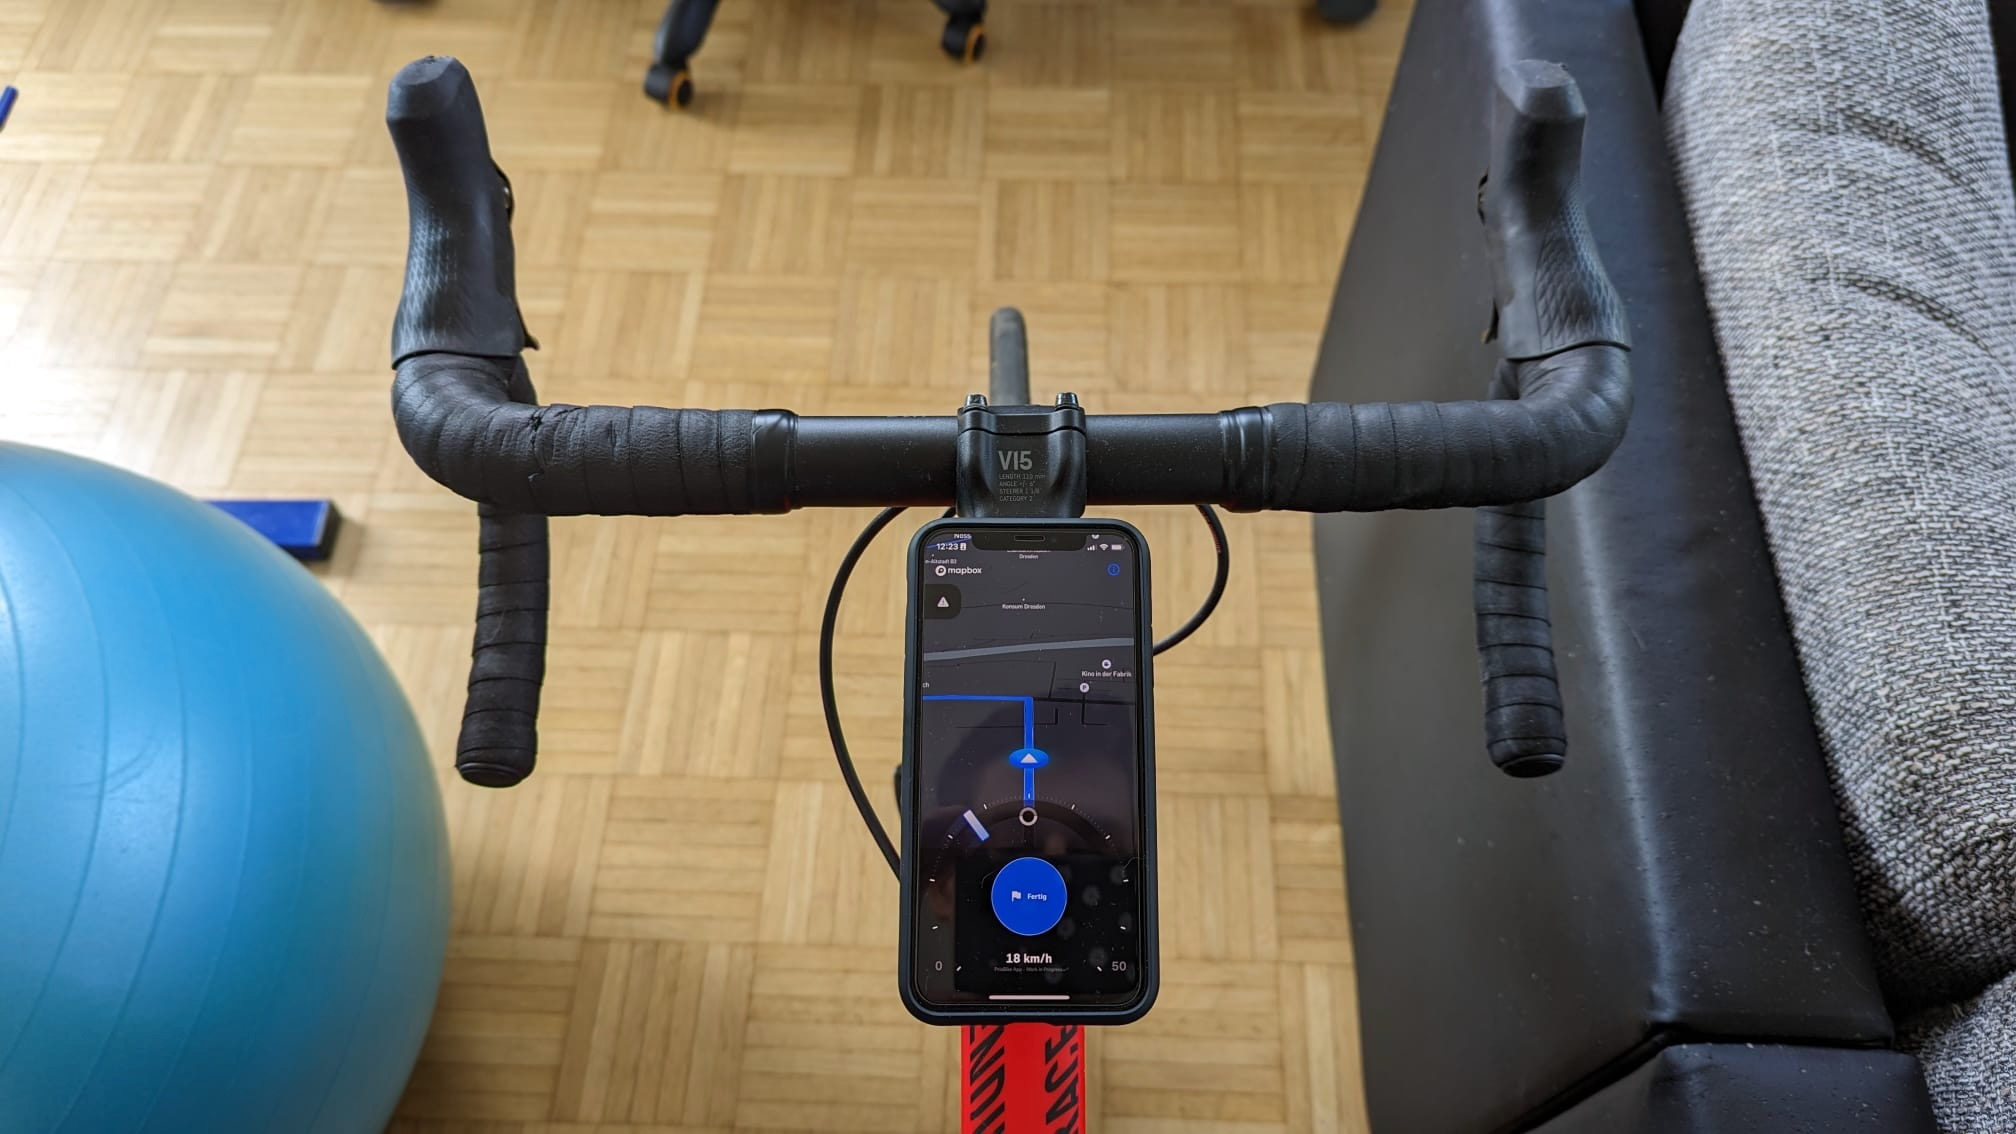
\includegraphics[width=\linewidth]{evaluation/Halterung_Philipp.jpeg}
\caption{Smartphone-Halterung von \philipp.}\label{fig:evaluation:philipp:halterung}
\end{figure}

\begin{figure}[]
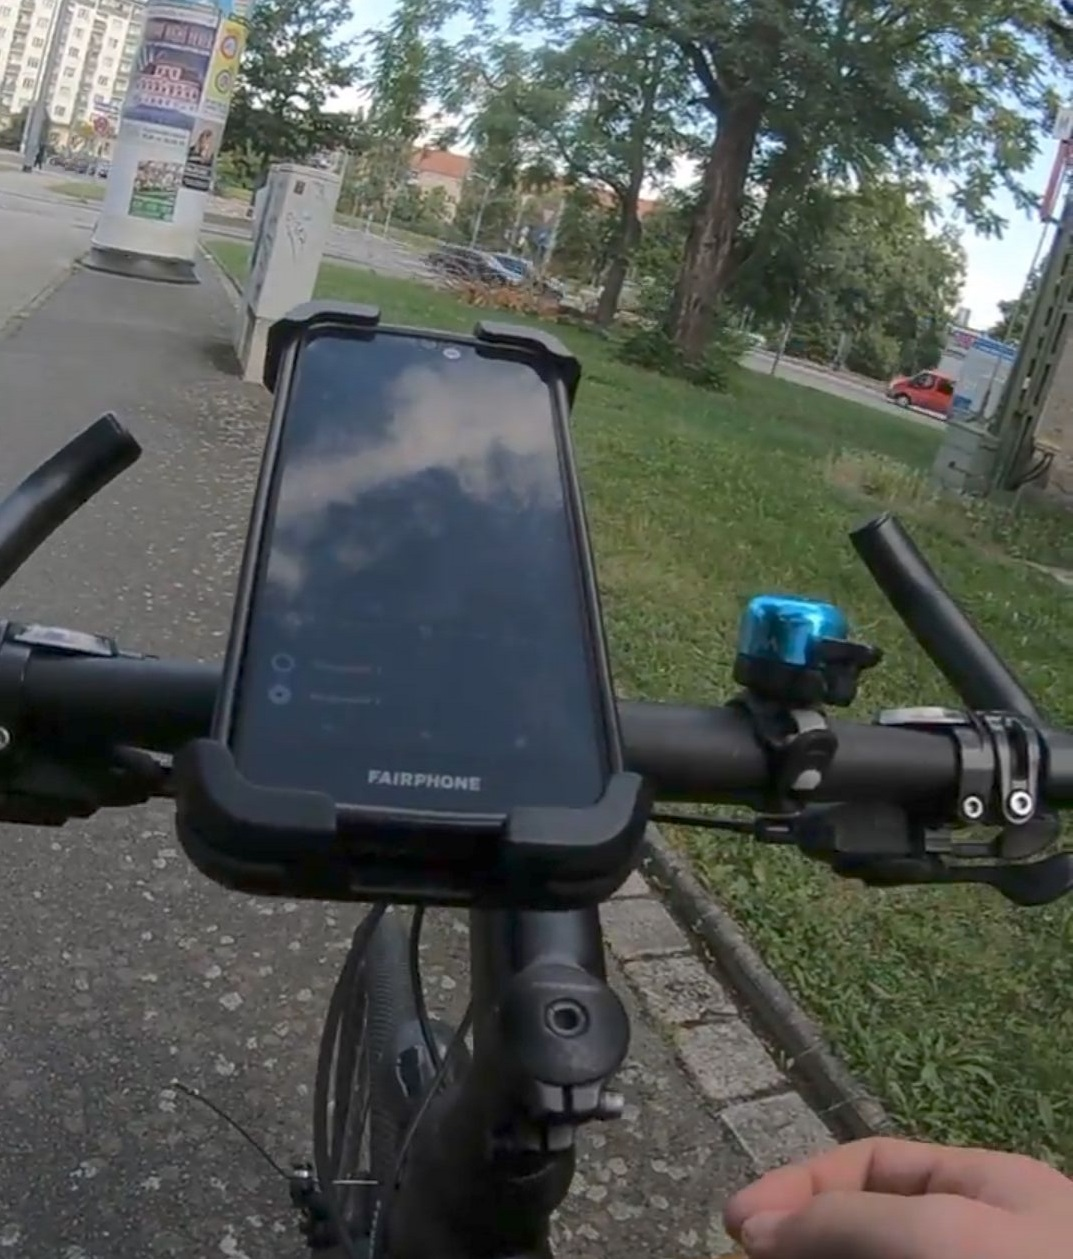
\includegraphics[width=0.5\linewidth]{evaluation/halterung.jpg}
\caption{Am Lenker befestigte Smartphone-Halterung von \florian. Person A und B verwenden eine ähnliche Halterung.}\label{fig:evaluation:default:halterung}
\end{figure}

Die Smartphones wurden mittels einer Halterung am Fahrrad befestigt. Person A, B und C verwendeten eine Halterung, welche am Lenker des Fahrrads befestigt wurde, wie sie beispielhaft in Abbildung \ref{fig:evaluation:default:halterung} zu sehen ist. Dabei wurde versucht, eine Reichweite von Blickwinkeln der Innenkamera des Smartphones auf die Person zu erzeugen, indem die Halterungen an anderen Stellen des Lenkers befestigt wurden. Person D verwendet eine Halterung, wodurch ein generell anderer Winkel auf die Person gegeben ist. Die Halterung ist in Abbildung \ref{fig:evaluation:philipp:halterung} zu sehen. Die Probanden haben für die Aufnahme der Videos unterschiedliche Geräte verwendet. Eine Übersicht über die verwendeten Geräte ist in Tabelle \ref{tab:evaluation:devices} zu sehen.

\begin{table}[]
\begin{tabular}{c l}
\toprule
\textbf{Person} & \textbf{Gerät} \\ \midrule
A      & Samsung Galaxy S10 \\
B      & Google Pixel 5     \\
C      & Fairphone 3+       \\
D      & iPhone XS     \\ \bottomrule    
\end{tabular}
\caption{Übersicht über die verwendeten Smartphones.}
\label{tab:evaluation:devices}
\end{table}

Es gab keine Vorgaben, wie sich die Personen auf dem Fahrrad verhalten sollten. Die Videos wurden jedoch mit dem Ziel aufgenommen, möglichst viele verschiedene Situationen darzustellen. So wurde darauf geachtet, dass möglichst viele verschiedene Wettersituationen, wie sonniges oder bewölktes Wetter, dargestellt werden. Es wurden auch Videos bei Nacht aufgenommen. Außerdem soll die Auswirkungen von Brillen untersucht werden. Daher gibt es Videos, in denen die Personen eine Brille oder Sonnenbrille tragen, sowie Videos, in denen keine Brille getragen wird. Zusätzlich ist zu beachten, dass in manchen Videos ein Verhalten simuliert wurde, das in realen Situationen wahrscheinlich nicht so auftreten würde. So neigt zum Beispiel \philipp in Video 10 den Kopf besonders stark zum Smartphone-Display, wenn die Person auf das Smartphone schaut.

Alle Videos wurden im MP4-Format gespeichert\footnote{Die Videos von \philipp (Video 9 und 10) wurden im MOV-Format gespeichert und vor der Verarbeitung des Videos in das MP4-Format konvertiert.}. Die Videos wurden im Hochformat mit einem Seitenverhältnis von 9:16 und mit einer Bildrate von 30 Bildern pro Sekunde aufgenommen\footnote{Das Video von Person C (Video 8) wurde mit 60 Bildern pro Sekunde aufgenommen und anschließend auf 30 Bilder pro Sekunde komprimiert.}. Die Videos haben eine Auflösung von $1080 \times 1920$ Pixel. Bei der Zerlegung der Videos in die einzelnen Frames ergeben sich insgesamt 67.017 Bilder. Wie in Kapitel \ref{sec:implemenation:video} erwähnt, wird davon nur jedes dritte Bild für die Evaluation verarbeitet. Insgesamt werden also 22.339 Frames in der Auswertung berücksichtigt. Eine Übersicht über die aufgenommen Videos ist in den Tabellen \ref{tab:evaluation:videos:1} und \ref{tab:evaluation:videos:2} dargestellt.

\begin{table}[]
\begin{tabular}{c c r p{2cm} p{4cm} c c}
\toprule
\textbf{Video} & \textbf{Person} & \textbf{Frames}  & \textbf{Datum} & \textbf{Besonderheiten} & \textbf{Wetter} & \textbf{Accessoire}     \\ \midrule
01   & A  & 1.427     & 26.08.2023, 17:22 Uhr &  & \Cloud & \tikz{\duck[invisible,squareglasses]}                       \\
02   & A  & 1.267     & 26.08.2023, 17:27 Uhr &  & \Cloud  & \tikz{\duck[invisible,squareglasses]}                     \\
03   & A  & 1.238     & 26.08.2023, 17:31 Uhr & & \Cloud & \tikz{\duck[invisible,squareglasses]}                      \\
04   & A  & 1.573     & 26.08.2023, 17:42 Uhr & Holpriger Untergrund & \Cloud & \tikz{\duck[invisible,squareglasses]} \\
05   & A  & 1.427     & 26.08.2023, 17:48 Uhr & Holpriger Untergrund & \Cloud & \tikz{\duck[invisible,squareglasses]} \\
06   & A  & 674       & 04.09.2023, 14:22 Uhr & Person in Ruhe, sitzend auf Bank  & \Sun\footnote{Person A befindet sich in einem ausgeleuchteten Raum.} &  \tikz{\duck[invisible,squareglasses]}                    \\
07   & B  & 2.623     & 05.09.2023, 13:53 Uhr &  & \Sun &  \tikz{\duck[invisible,sunglasses]}  \\
08   & C  & 3.596     & 05.09.2023, 17:22 Uhr & Helm & \Sun & \\
09   & D  & 4.922     & 05.09.2023, 17:42 Uhr & Helm, Halterungsposition & \Sun & \\
10  & D  & 3.268     & 05.09.2023, 17:46 Uhr & Helm, Halterungsposition, Versucht mit Kopfrotation auf Gerät zu schauen & \Sun & \tikz{\duck[invisible,sunglasses]} \\
11  & A  & 7.098     & 06.09.2023, 11:32 Uhr &  & \Sun & \tikz{\duck[invisible,squareglasses]}\footnote{Person A nimmt die Brille während der Fahrt ab.}  \\
12  & A  & 4.684     & 06.09.2023, 11:36 Uhr & Holpriger Untergrund & \Sun & \tikz{\duck[invisible,squareglasses]}   \\
13  & A  & 9.172     & 06.09.2023, 11:41 Uhr & Holpriger Untergrund & \Sun & \tikz{\duck[invisible,squareglasses]} \\
14  & A  & 3.744     & 06.09.2023, 11:46 Uhr & sehr sonnig & \Sun & \tikz{\duck[invisible,squareglasses]}\\
15  & A  & 2.334     & 06.09.2023, 11:48 Uhr & sehr sonnig& \Sun & \\
16  & A  & 785       & 06.09.2023, 11:51 Uhr &  & \Sun & \tikz{\duck[invisible,squareglasses]}\\
17  & A  & 2.448     & 06.09.2023, 11:57 Uhr & Halterungsposition & \Sun &  \\
18  & A  & 2.525     & 08.09.2023, 09:32 Uhr &  & \Sun & \\
19  & A  & 1.568     & 08.09.2023, 10:01 Uhr &  & \Sun &  \\
\bottomrule
\end{tabular}
\caption{Teil 1 der Übersicht über die aufgenommenen Videos. Die Übersicht zeigt die dargestellte Person, die Anzahl der Bilder des Videos, den Aufnahmezeitpunkt sowie Besonderheiten, die in diesem Video zu sehen sind. Außerdem wird das Wetter angezeigt. \Cloud\xspace bedeutet bewölkter Himmel. \Sun\xspace bedeutet sonniges Wetter. \leftmoon bedeutet klarer Nachthimmel. Außerdem werden Accessoires gezeigt, die von den dargestellten Personen getragen werden. \protect\tikz{\duck[invisible,squareglasses]} bedeutet, dass die Person eine Brille trägt. \protect\tikz{\duck[invisible,sunglasses]} bedeutet, dass die Person eine Sonnenbrille trägt.}
\label{tab:evaluation:videos:1}
\end{table}

\begin{table}[]
\begin{tabular}{c c r p{2cm} p{4cm} c c}
\toprule
\textbf{Video} & \textbf{Person} & \textbf{Frames}  & \textbf{Datum} & \textbf{Besonderheiten} & \textbf{Wetter} & \textbf{Accessoire}     \\ \midrule
20  & A  & 3.250     & 08.09.2023, 13:44 Uhr &  & \Sun & \tikz{\duck[invisible,squareglasses]} \\
21  & A  & 2.315     & 08.09.2023, 13:47 Uhr &  & \Sun & \tikz{\duck[invisible,squareglasses]} \\
22  & A  & 1.893     & 10.09.2023, 20:22 Uhr & sehr dunkle Umgebung & \leftmoon & \tikz{\duck[invisible,squareglasses]}\\
23  & A  & 1.450     & 10.09.2023, 20:37 Uhr & dunkle Umgebung, vereinzelt Laternen  & \leftmoon & \tikz{\duck[invisible,squareglasses]}\\
24  & A  & 1.736     & 10.09.2023, 20:41 Uhr & dunkle Umgebung, ausgeleuchtete Hauptstraße & \leftmoon & \tikz{\duck[invisible,squareglasses]} \\
\bottomrule
\end{tabular}
\caption{Teil 2 der Übersicht über die Videos.}
\label{tab:evaluation:videos:2}
\end{table}

\subsection{Erstellung Ground Truth}\label{sec:evaluation:ground:truths}

In der Evaluation soll untersucht werden, zu welchen Zeitpunkten die Person auf das Smartphone sieht. Um dafür einen Vergleichswert zu haben, muss eine Ground Truth für die einzelnen Frames erstellt werden, die angibt, ob eine Person auf das Smartphone sieht oder nicht. Wie in Kapitel \ref{sec:implemenation:video} beschrieben, werden dafür die einzelnen Frames des Videos als Bild gespeichert. Während der Aufnahme der Videos war es nicht möglich, die Ground Truth automatisiert zu erstellen. Wie in der Arbeit von Smith et al. \cite{paper:columbia} erwähnt, können wir Menschen jedoch sehr gut erkennen, ob eine Person uns ansieht oder nicht. Die bearbeiteten Bilder der Videos sollen daher von einem Menschen annotiert werden. Die Bilder können in eine der drei folgenden Kategorien eingeordnet werden:

\begin{itemize}
\item A.0) Person sieht nicht auf das Gerät (siehe Abbildung \ref{fig:evaluation:gaze:no}).
\item A.1) Person sieht auf das Gerät (siehe Abbildung \ref{fig:evaluation:gaze:yes}).
\item A.2) Augen oder Gesicht der Person sind nicht im Bild (siehe Abbildung \ref{fig:evaluation:gaze:not_sure}).
\end{itemize}

\begin{figure}{}
    \begin{subfigure}{0.3\textwidth}
        
\includegraphics[width=\linewidth]{evaluation/sieht_nicht_0.jpg}
        \caption{Person sieht nicht auf das Smartphone.}
        \label{fig:evaluation:gaze:no}
    \end{subfigure}
    \begin{subfigure}{0.3\textwidth}
        
\includegraphics[width=\linewidth]{evaluation/sieht_nicht_1.jpg}
        \caption{Person sieht auf das Smartphone.}
        \label{fig:evaluation:gaze:yes}
    \end{subfigure}
    \begin{subfigure}{0.3\textwidth}
        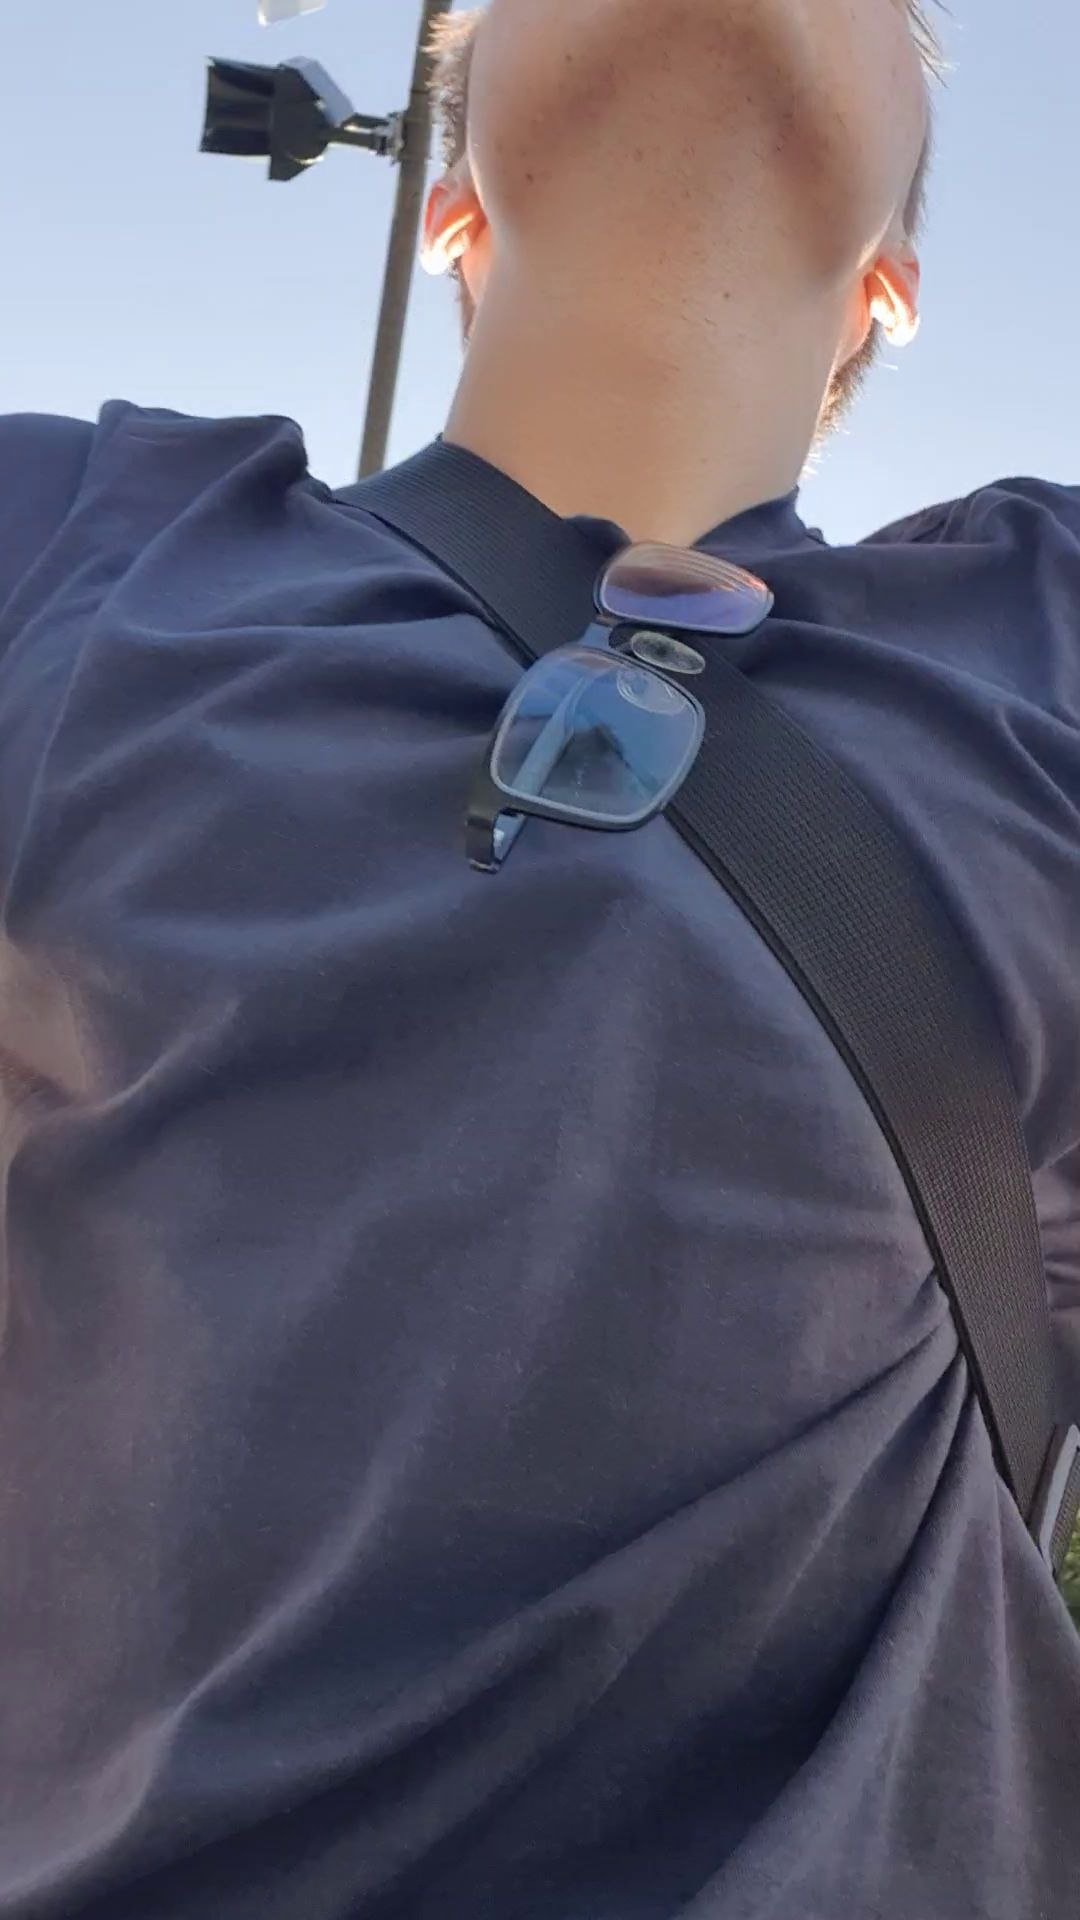
\includegraphics[width=\linewidth]{evaluation/sieht_nicht_2.jpg}
        \caption{Gesicht von Person ist außerhalb des Bildes.}
        \label{fig:evaluation:gaze:not_sure}
    \end{subfigure}
    \caption{Beispiel für die einzelnen Kategorien der Ground Truth für den Blickkontakt einer Person mit dem Display eines Smartphones.}
    \label{fig:evaluation:gaze:labels}
\end{figure}

Dabei wird angenommen, dass wenn das Gesicht der Person nicht erkennbar ist, die Person auch nicht auf das Smartphone sieht. 

Weiter soll bei der Evaluation ein Grenzwert für das \textit{Eye Aspect Ratio} ($EAR$) bestimmt werden, um geschlossene Augen erkennen zu können. Dafür muss für jedes dieser Bilder zusätzlich entschieden werden, ob die Augen der Person geschlossen sind. Jedes Bild wird dabei einer der folgenden Kategorien zugeordnet:

\begin{itemize}
    \item B.0) Augen geschlossen (siehe Abbildung \ref{fig:evaluation:eye:closed})
    \item B.1) Augen geöffnet (siehe Abbildung \ref{fig:evaluation:eye:open})
    \item B.2) Augen nicht erkenntlich (siehe Abbildung \ref{fig:evaluation:eye:not_sure})
\end{itemize}

\begin{figure}{}
    \begin{subfigure}{0.3\textwidth}
        
\includegraphics[width=\linewidth]{evaluation/auge_geschlossen.jpg}
        \caption{Augen der Person sind geschlossen.}
        \label{fig:evaluation:eye:closed}
    \end{subfigure}
    \begin{subfigure}{0.3\textwidth}
        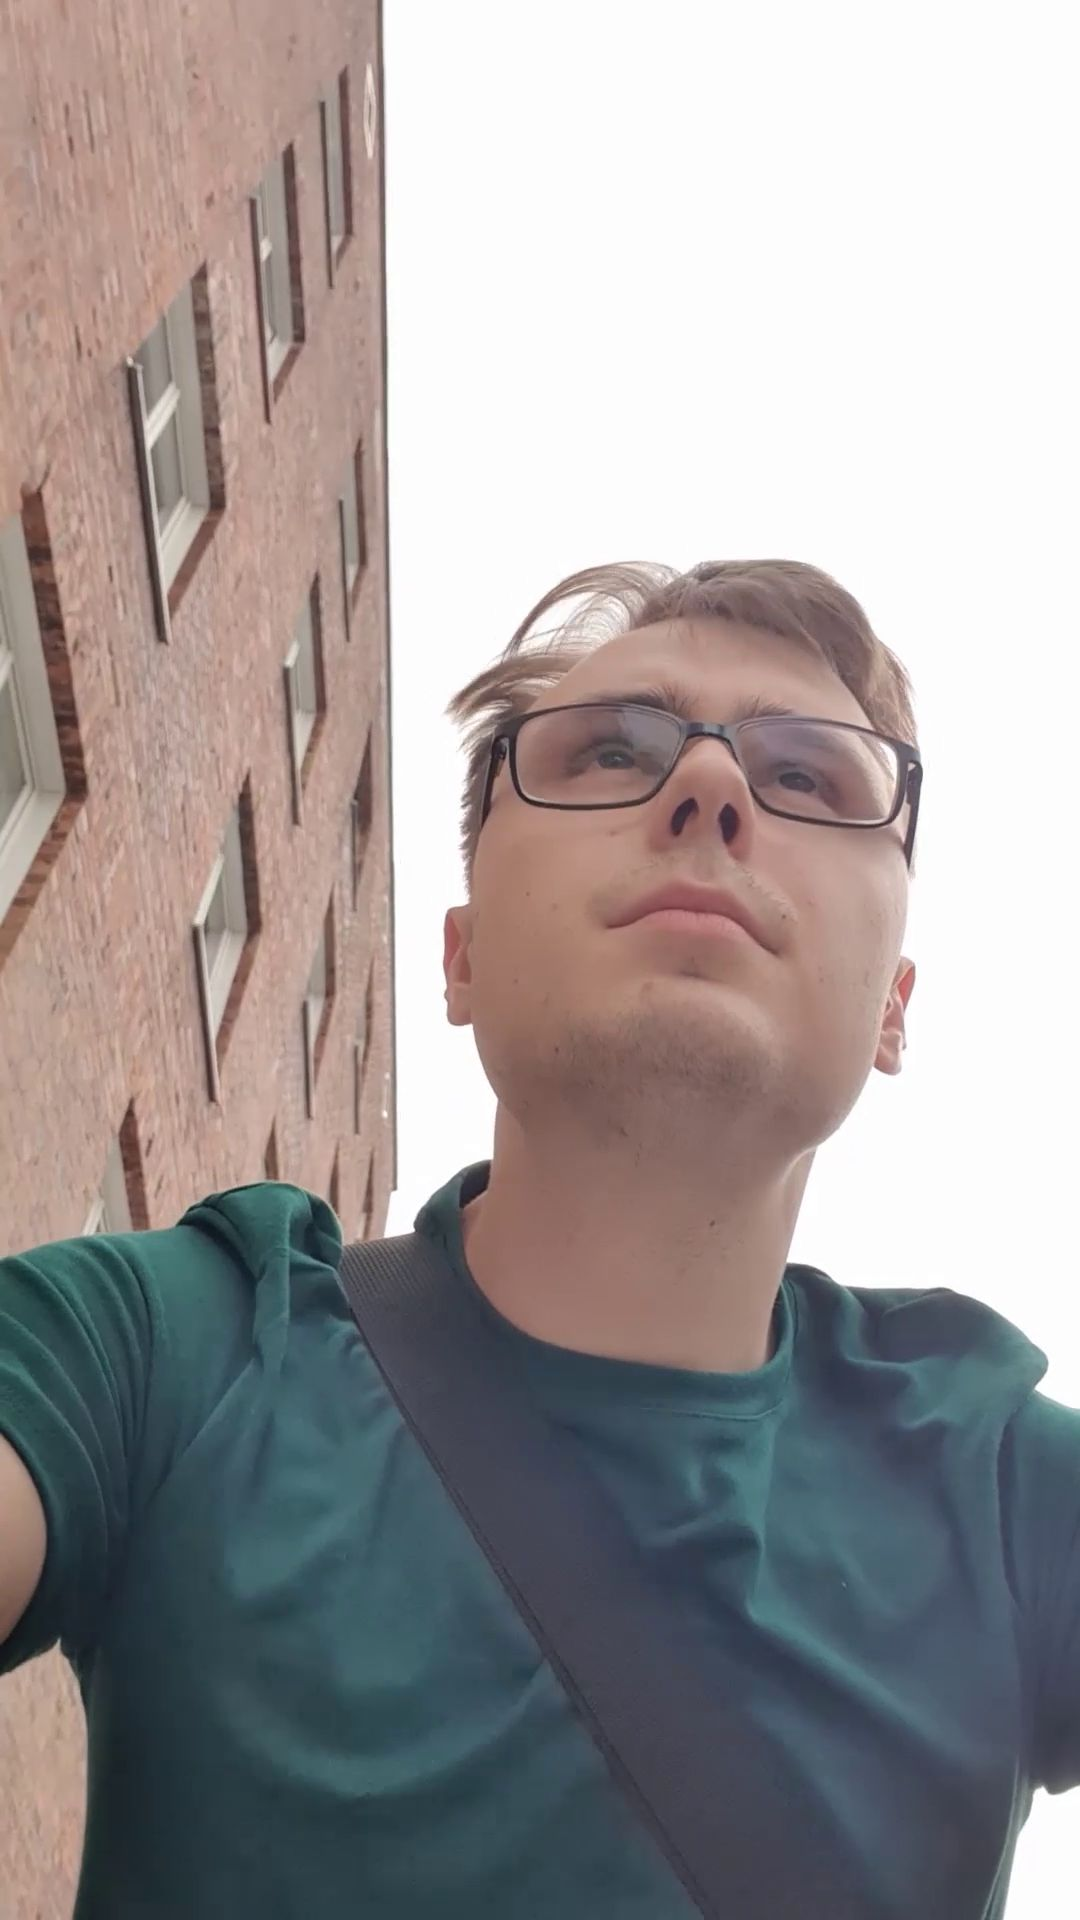
\includegraphics[width=\linewidth]{evaluation/auge_offen.jpg}
        \caption{Augen der Person sind geöffnet.}
        \label{fig:evaluation:eye:open}
    \end{subfigure}
    \begin{subfigure}{0.3\textwidth}
        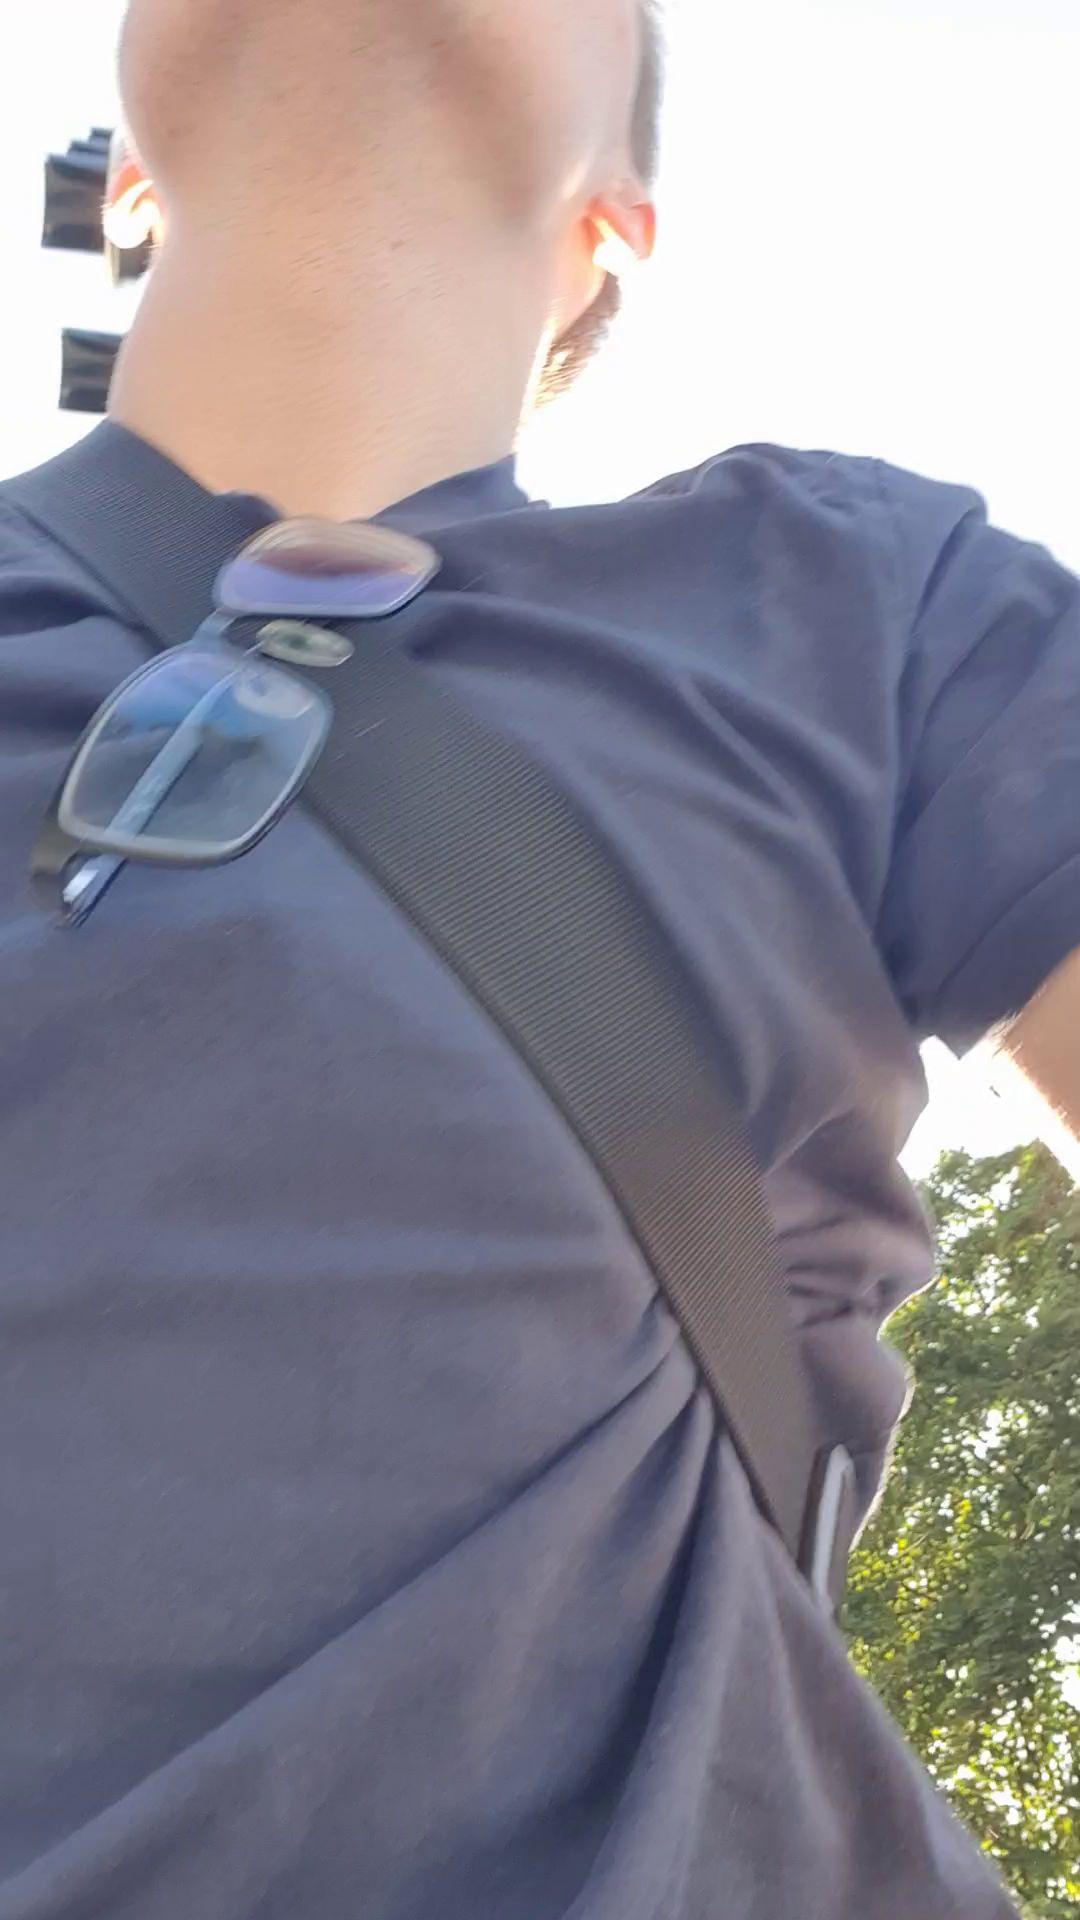
\includegraphics[width=\linewidth]{images/evaluation/auge_none.jpg}
        \caption{Augen der Person sind außerhalb des Bildes.}
        \label{fig:evaluation:eye:not_sure}
    \end{subfigure}
    \caption{Beispiel für die einzelnen Kategorien der Ground Truth für den Blickkontakt einer Person mit dem Display eines Smartphones.}
    \label{fig:evaluation:eye:labels}
\end{figure}


Für die Erstellung der Ground Truth wurde eine kleine Gruppe von Personen ausgewählt und instruiert. Diese Gruppe von Personen hat dann das Kategorisieren der Bilder durchgeführt. Um menschliche Fehler zu vermeiden, wurde der Prozess nach Abschluss des ersten Durchgangs wiederholt. Unterschiede zwischen dem ersten und dem zweiten Durchgang wurden anschließend in der Gruppe diskutiert und entschieden. 

Da sowohl die Ground Truth für den Blickkontakt als auch für die Erkennung von geschlossenen Augen aus drei Kategorien bestehen, können diese in einem gemeinsamen Dateiformat gespeichert werden. Dafür wird jeder Kategorie ein numerischer Wert zwischen 0 und 2 zugeordnet. Die genaue Zuordnung ist in Tabelle \ref{tab:evaluation:labels:numeric:values} dargestellt. Die Ergebnisse werden dann in einer Datei gespeichert. Ein Ausschnitt einer solchen Datei ist in Abbildung \ref{code:evaluation:labels:output} dargestellt. Für jeden Frame des Videos wird ein eigener Eintrag in der entsprechenden Datei erzeugt. Dieser besteht aus der Nummer des Frames $n$ und dem entsprechenden numerischen Wert der Kategorie, welche durch ein Semikolon getrennt werden. Wenn für einen Frame noch keine Kategorie festgelegt wurde, erhält dieser Frame den Wert 3. Am Anfang der Datei steht ein Wahrheitswert, der angibt, ob allen vorhandenen Bildern eine Kategorie zugewiesen wurde.

\begin{table}[]
    \centering
    \begin{tabular}{c c c}
    \toprule
         \textbf{Wert} & \makecell{\textbf{Ground Truth}\\\textbf{Blickkontakt}} & \makecell{\textbf{Ground Truth}\\\textbf{Augen geöffnet}} \\ \midrule
         0 & A.0 & B.0 \\
         1 & A.1 & B.1 \\
         2 & A.2 & B.2 \\
         \bottomrule
    \end{tabular}
    \caption{Numerischer Wert der Kategorien der beiden Ground Truths.}
    \label{tab:evaluation:labels:numeric:values}
\end{table}

\begin{figure}
    \centering
   \begin{lstlisting}[language=Java]
false // Nicht alle Frames des Videos wurden in eine Kategorie eingeordnet
0;0 // Der Frame mit der Nummer 0 gehoert zur Kategorie 0
3;1 // Der Frame mit der Nummer 3 gehoert zur Kategorie 1
6;0
9;2 // Der Frame mit der Nummer 9 gehoert zur Kategorie 2
12;3 // Fuer den Frame 12 wurde noch keine Kategorie festgelegt
15;3 
...
\end{lstlisting}
    \caption{Ausschnitt einer Datei die Ground Truth Daten enthält.}
    \label{code:evaluation:labels:output}
\end{figure}


\subsection{Qualität der Gesichtserkennung}\label{sec:evaluation:plan:quality:face}

Wie bereits in Kapitel \ref{sec:concept:head} diskutiert, muss für eine genaue Auswertung der Gesichtserkennung die mittlere Abweichung der erkannten Gesichtsmerkmale von ihrer tatsächlichen Position \cite{paper:evaluation-face} bestimmt werden. Im Rahmen dieser Arbeit würde dies bedeuten, dass für alle 22.339 verarbeiteten Bilder die tatsächliche Position einiger markanter Gesichtspunkte manuell im Bild markiert werden muss. Dies war im zeitlichen Rahmen dieser Arbeit nicht realisierbar. Daher wurde entschieden, die Gesichtserkennung qualitativ zu bewerten. Dazu wurden, wie in Kapitel \ref{sec:implementation:face:export:landmarks} beschrieben, während der Verarbeitung der Videos die Bilder der erkannten Gesichter mit den markierten Gesichtspunkten gespeichert. Zur besseren Übersicht wurden markante Punkte im Gesicht farblich hervorgehoben, um die Qualitätsbeurteilung zu erleichtern. Die Bilder mit den erkannten Gesichtern wurden dann manuell in eine der drei folgenden Kategorien eingeordnet:  

\begin{itemize}
\item Gut erkannt (siehe Abbildungen \ref{fig:evaluation:face:dlib:good} und \ref{fig:evaluation:face:mediapipe:good})
\item Ungenau erkannt (siehe Abbildungen \ref{fig:evaluation:face:dlib:medium} und \ref{fig:evaluation:face:mediapipe:medium})
\item Schlecht erkannt (siehe Abbildungen \ref{fig:evaluation:face:dlib:bad} und \ref{fig:evaluation:face:mediapipe:medium})
\end{itemize}

Indirekt kann noch eine vierte Kategorie abgeleitet werden, die Bilder beinhaltet, in denen kein Gesicht erkannt werden konnte.

Um eine einheitliche Bewertung zu gewährleisten, wurden alle erkannten Gesichter von derselben Person bewertet. 

\begin{figure}{}
    \begin{subfigure}{0.33\textwidth}
        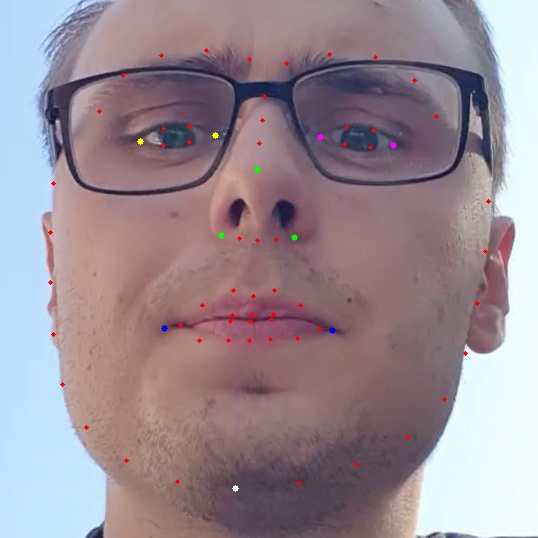
\includegraphics[width=0.9\linewidth]{evaluation/dlib_gute_erkennung.jpg}
        \caption{Gut erkannte Gesichtsmerkmale (dlib)}
        \label{fig:evaluation:face:dlib:good}
    \end{subfigure}%
    \begin{subfigure}{0.33\textwidth}
        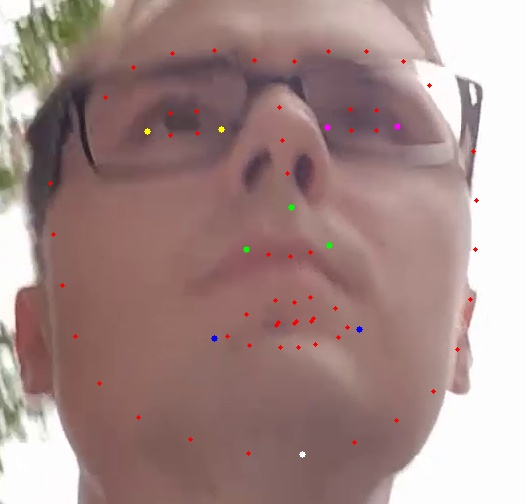
\includegraphics[width=0.9\linewidth]{evaluation/dlib_ungenaue_erkennung.jpg}
        \caption{Ungenau erkannte Gesichtsmerkmale (dlib)}
        \label{fig:evaluation:face:dlib:medium}
    \end{subfigure}
    \begin{subfigure}{0.33\textwidth}
        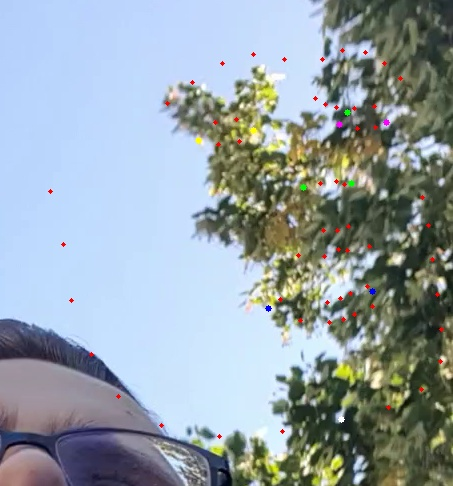
\includegraphics[width=0.9\linewidth]{evaluation/dlib_schlechte_erkennung.jpg}
        \caption{Schlecht erkannte Gesichtsmerkmale (dlib)}
        \label{fig:evaluation:face:dlib:bad}
    \end{subfigure}
    \begin{subfigure}{0.33\textwidth}
        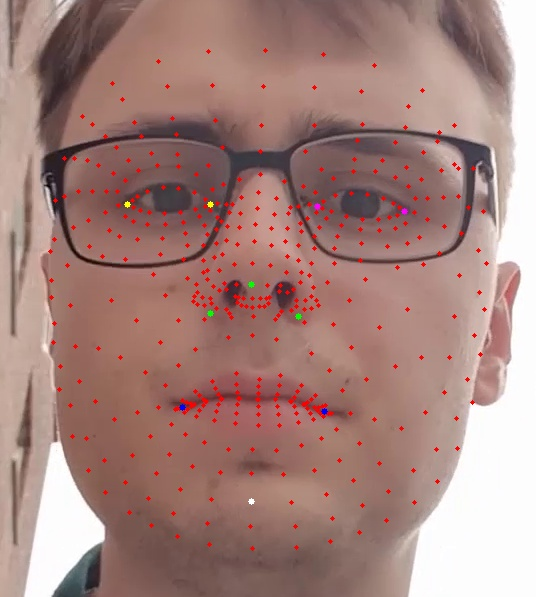
\includegraphics[width=0.9\linewidth]{evaluation/mediapipe_gute_erkennung.jpg}
        \caption{Gut erkannte Gesichtsmerkmale (MediaPipe)}
        \label{fig:evaluation:face:mediapipe:good}
    \end{subfigure}%
    \begin{subfigure}{0.33\textwidth}
        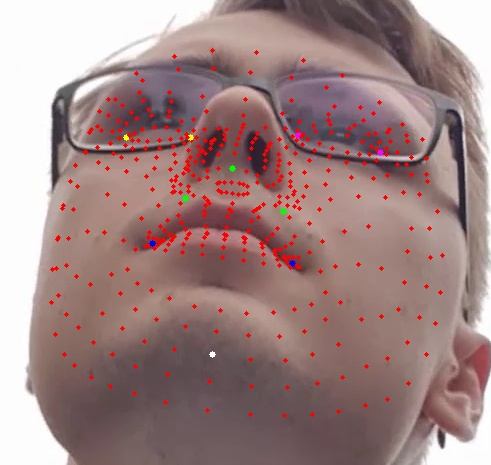
\includegraphics[width=0.9\linewidth]{evaluation/mediapipe_ungenaue_erkennung.jpg}
        \caption{Ungenau erkannte Gesichtsmerkmale (MediaPipe)}
        \label{fig:evaluation:face:mediapipe:medium}
    \end{subfigure}
    \begin{subfigure}{0.33\textwidth}
        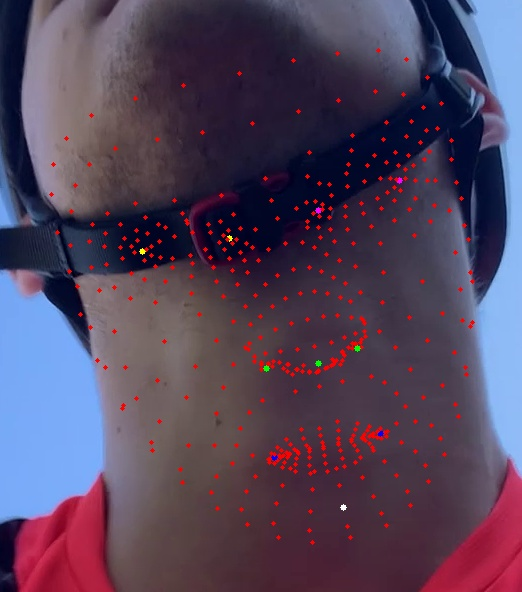
\includegraphics[width=0.9\linewidth]{evaluation/mediapipe_schlecht_erkennung.jpg}
        \caption{Schlecht erkannte Gesichtsmerkmale (MediaPipe)}
        \label{fig:evaluation:face:mediapipe:bad}
    \end{subfigure}
    \caption{Beispiele für verschiedene Qualitäten der erkannte Gesichter von \dlib und \mediapipe.}
    \label{fig:evaluation:face}
\end{figure}

\subsection{Webanwendung für die Evaluation}\label{sec:evaluation:plan:tool}

Für die Evaluation wurde eine Webanwendung mit Angular\footnote{\url{https://angular.io/} (Abgerufen am 31.10.2023)} entwickelt. Sie besteht aus zwei Ansichten. Zum einen gibt es eine Ansicht, die für die Erstellung der Ground Truth entwickelt wurde. Zum anderen gibt es eine Ansicht, mit der die Ergebnisse der Gesichtserkennung und der Blickrichtungsbestimmung visualisiert werden können, um so mögliche Fehlerquellen zu identifizieren und zu verstehen. Beide Ansichten werden im Folgenden näher vorgestellt.

\subsubsection{Ansicht Ground Truth}

Für die effiziente Erstellung der Ground Truth sowohl für Blickkontakt als auch für geschlossene Augen wurde eine Ansicht erstellt. Ein Beispiel für diese Ansicht ist in Abbildung \ref{fig:evaluation:tool} dargestellt. In der Mitte der Ansicht ist das aktuelle Bild zu sehen. Links und rechts davon befinden sich zwei große Schaltflächen. Der linke rote Button speichert je nach aktueller Auswahl die Kategorie A.0 oder B.0 für das angezeigte Bild. Der rechte grüne Knopf wird für die Kategorien A.1 und B.1 verwendet. Die Sonderfälle A.2 und B.2 können durch die Schaltfläche mit dem Fragezeichen markiert werden. Durch Drücken einer der Schaltflächen wird die entsprechende Kategorie für das Bild gespeichert und automatisch das nächste Bild des Videos geladen.
Diese Ansicht wurde auch verwendet, um die Qualität der Gesichtserkennung zu bewerten.

\begin{figure}[]
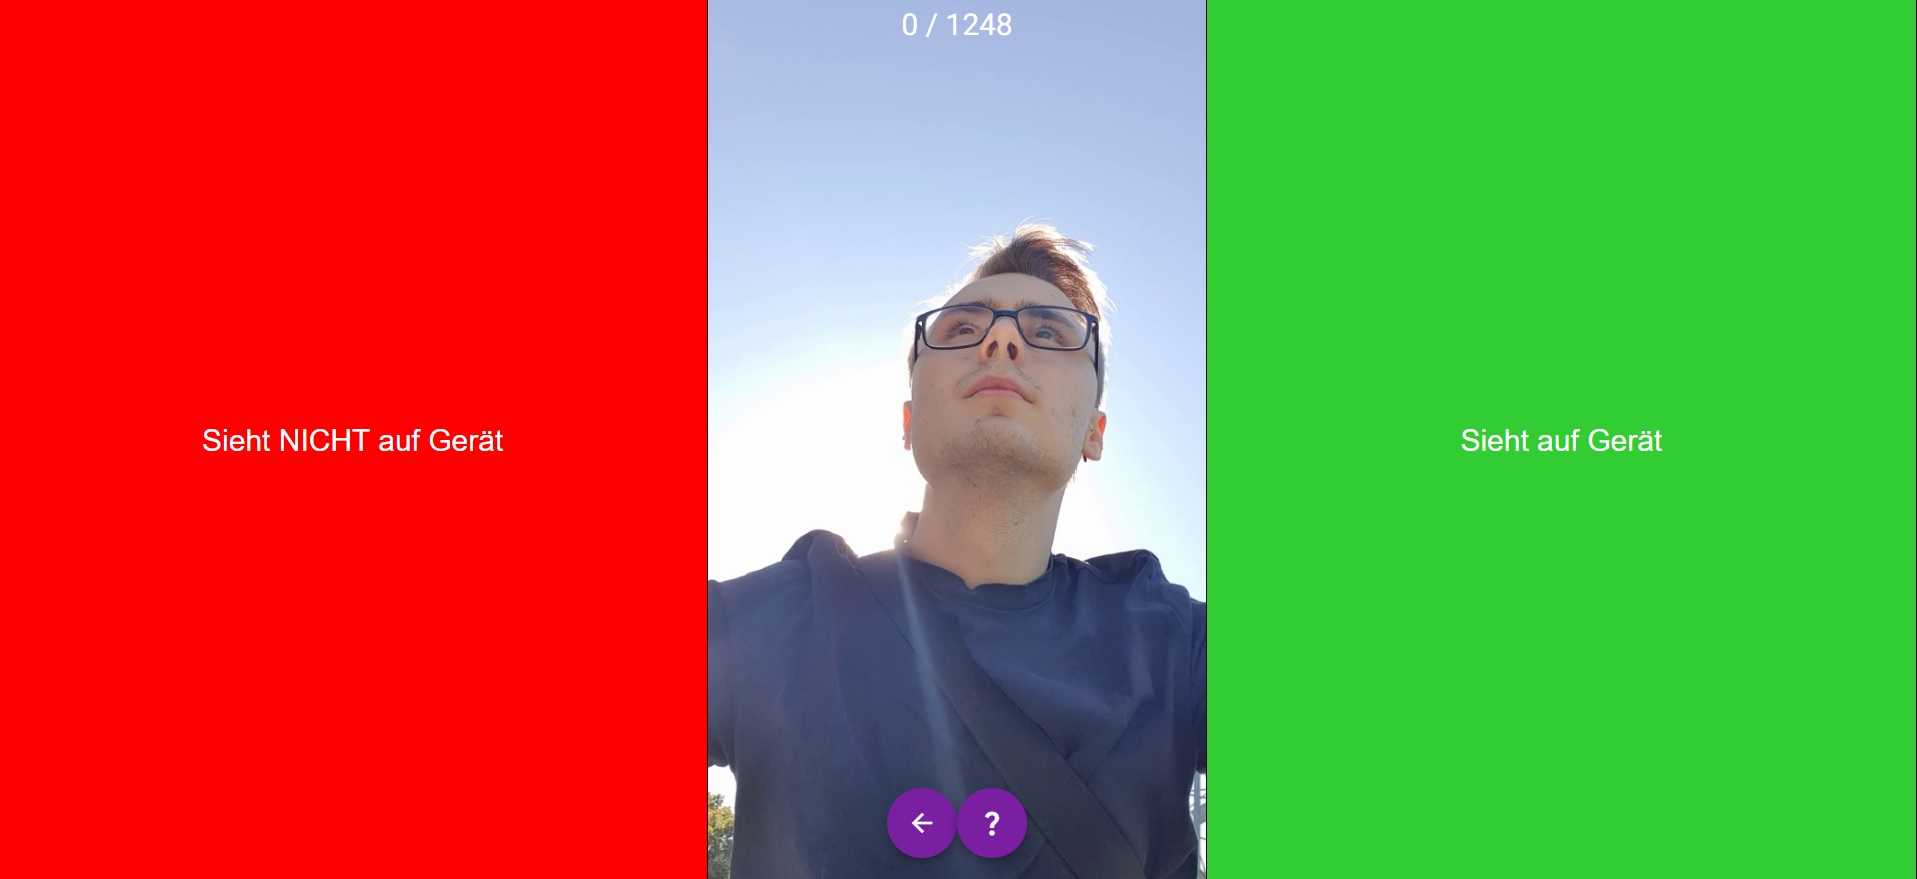
\includegraphics[width=\linewidth]{evaluation/tool.jpg}
\caption{Ansicht zur Kategorisierung eines einzelnen Frames.}\label{fig:evaluation:tool}
\end{figure}

\subsubsection{Ansicht Analyse}

In der Ansicht zur Analyse der Ergebnisse werden verschiedene Daten, die während der Verarbeitung eines Frames gesammelt wurden, für eine gemeinsame Betrachtung zusammengestellt. Die Ansicht ist in Abbildung \ref{fig:evaluation:debug} zu sehen. Auf der linken Seite der Ansicht befindet sich das Originalbild des aktuellen Frames. Im unteren Teil der Ansicht wird die Ground Truth des Blickkontakts in Worten angezeigt, um gegebenenfalls ein falsch zugeordnetes Bild zu erkennen.  Im unteren Teil der rechten Seite ist ein Bild des erkannten Gesichts mit den zugehörigen Gesichtspunkten zu sehen, das während der Verarbeitung gespeichert wurde. Im mittleren Teil der Ansicht ist eine dreidimensionale Szene dargestellt. Zur Berechnung dieser Szene wurde die JavaScript-Bibliothek \textit{three.js}\footnote{\url{https://threejs.org/} (Abgerufen am 25.09.2023)} verwendet. In dieser Szene sind folgende Elemente zu sehen:

\begin{itemize}
    \item die berechnete dreidimensionale Position der Gesichtspunkte relativ zur Kamera,
    \item die Ebene $\cameraplane$,
    \item die Zone auf der Ebene $\cameraplane$, die das virtuelle Smartphone darstellt,
    \item die Sichtlinie der abgebildeten Person, berechnet aus dem Zentrum des Kopfes $\centerface$ und dem Blickrichtungsvektor $\gazevector$. 
\end{itemize}

Durch Knöpfe am unteren rechten Teil der Ansicht kann zwischen den einzelnen Frames des Videos gewechselt werden.

\begin{figure}
    \centering
    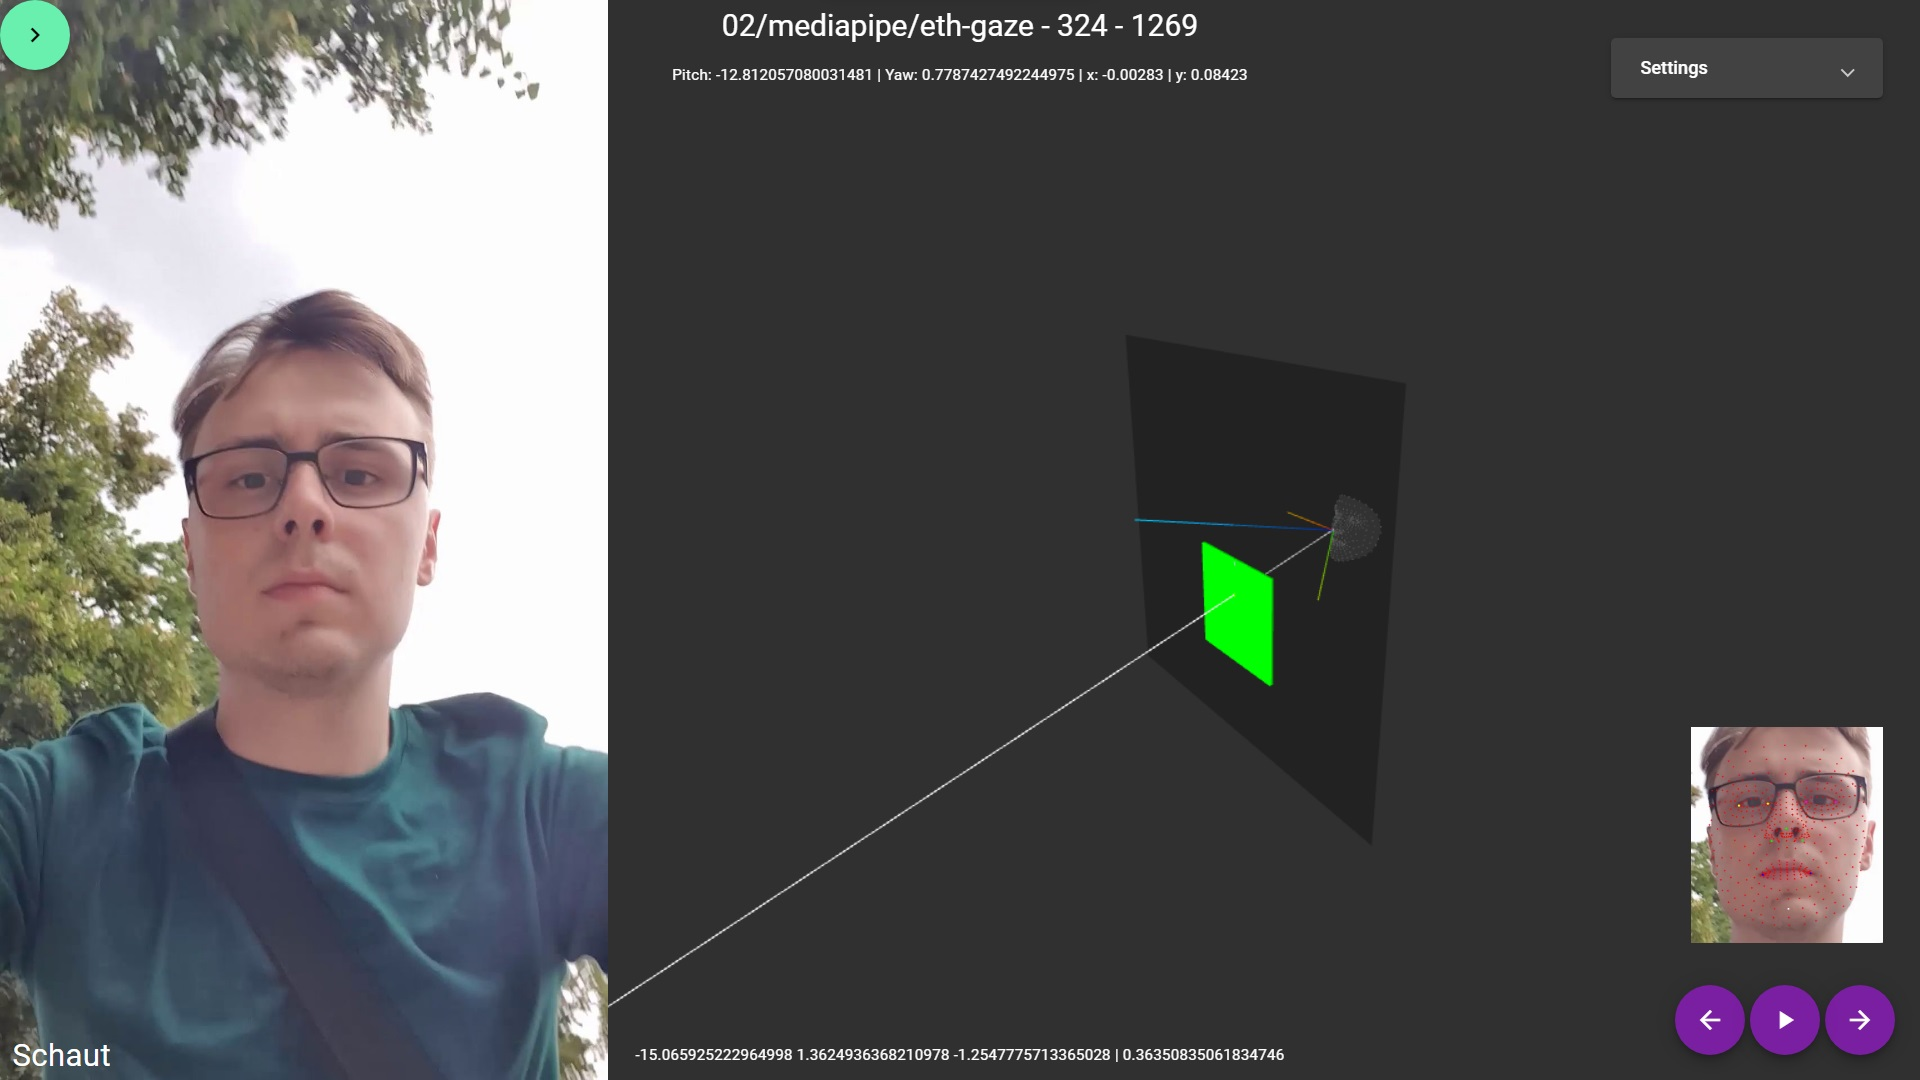
\includegraphics[width=\linewidth]{debug.jpg}
    \caption{Ansicht zur Analyse der Gesichtserkennung und Blickrichtungsbestimmung.}
    \label{fig:evaluation:debug}
\end{figure}

\section{Ergebnisse}\label{sec:evaluation:results}

In diesem Kapitel werden die Ergebnisse der Evaluation vorgestellt. Zunächst werden die Ergebnisse der Gesichtserkennung mit \dlib und \mediapipe diskutiert. Anschließend werden die Erkenntnisse der Analyse der Blickrichtungsbestimmung vorgestellt.

\subsection{Ergebnisse Gesichtserkennung}\label{sec:evaluation:results:face}

\begin{figure}
    \centering
    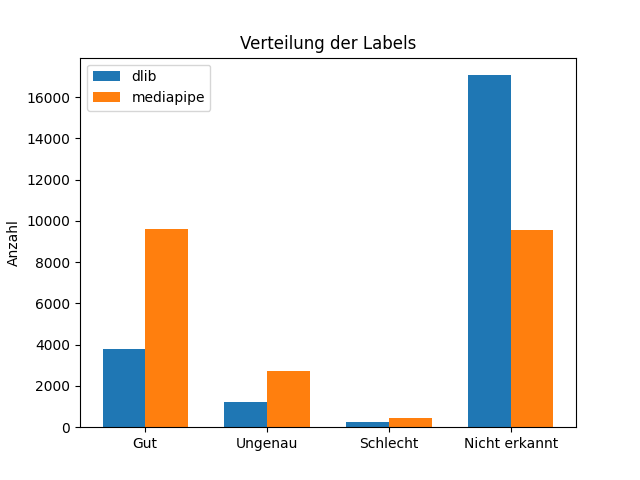
\includegraphics[width=0.7\linewidth]{evaluation/total-bar-quality.png}
    \caption{Gesamtzahl der Vorkommen der einzelnen Kategorien für \dlib und \mediapipe.}
    \label{fig:evaluation:total:quality}
\end{figure}

Nachdem die Qualität der Gesichtserkennung manuell bewertet wurde, können die Ergebnisse der beiden Gesichtserkennungsmethoden \dlib und \mediapipe verglichen werden. Abbildung \ref{fig:evaluation:total:quality} zeigt die Gesamtzahl der Vorkommen der einzelnen Kategorien sowohl für \dlib als auch für \mediapipe. Es ist zu erkennen, dass \mediapipe generell in deutlich mehr Bildern ein Gesicht erkennt als \dlib. Die genauen Vorkommen der Kategorien in den einzelnen Videos sind im Anhang zu finden.

Um die Gesamtqualität der erkannten Gesichter zwischen den Videos vergleichen zu können, wird der \textit{Qualitätsscore} eingeführt. Dazu wird zunächst eine Funktion $q$ definiert, die der Qualitätskategorie eines Frames einen numerischen Wert zuteilt. Die Funktion $q$ kann wie folgt beschrieben werden:

\[
q(Kategorie) = 
\begin{cases} 
0 & \text{wenn } Kategorie = schlecht \\
0,5 & \text{wenn } Kategorie = ungenau \\
1 & \text{wenn } Kategorie = gut \\
\end{cases}
\]

Der \textit{Qualitätsscore} ist dann der Durchschnitt der ermittelten Werte für alle erkannten Gesichter des Videos. 

In Kapitel \ref{sec:concept:head} wurde die These aufgestellt, dass wenn kein Gesicht im Bild erkannt werden kann, die Person auch nicht auf das Smartphone schaut. Dies wird vermutet, da erste Tests gezeigt haben, dass die Gesichtserkennung umso schlechter wird, je weiter der Kopf entlang der Querachse nach oben gedreht wird. Dies ist der Fall, wenn Radfahrende auf den Straßenverkehr schauen. Wenn sie jedoch auf ihr Smartphone schauen, neigen sie ihren Kopf in Richtung des Smartphone-Displays, wodurch die Gesichtserkennung besser funktioniert. Diese These soll in der Auswertung überprüft werden, indem untersucht wird, in wie vielen Bildern, in denen die Person auf das Smartphone schaut, ein Gesicht erkannt werden kann. Dazu wird der Bewertungsfaktor $\lambda$ eingeführt. Dieser gibt den prozentualen Anteil der Bilder, bei denen die Person auf das Smartphone schaut und gleichzeitig ein Gesicht erkannt wird ($N_{\text{Smartphone, Gesicht}}$), an der Gesamtzahl der Bilder an, bei denen die Person auf das Smartphone schaut ($N_{\text{Smartphone}}$). 

\[
\lambda = \frac{N_{\text{Smartphone,Gesicht}}}{N_{\text{Smartphone}}}\cdot 100
\]

Ein Wert von 100\% bedeutet, dass jedes Mal, wenn die Person auf das Smartphone geschaut hat, ein Gesicht erkannt werden konnte. Ein Wert von 0\% bedeutet, dass in keinem der Bilder, in denen die Person auf das Smartphone schaut, ein Gesicht erkannt werden konnte.

Die Tabelle \ref{tab:evaluation:face:scores} gibt einen Überblick über die Gesichtserkennung der einzelnen Videos. In der Tabelle wird angegeben:

\begin{itemize}
    \item der prozentuale Anteil der Bilder, in denen die Person auf das Smartphone sieht,
    \item der prozentuale Anteil der Bilder, in denen ein Gesicht erkannt wurde,
    \item der Wert $\lambda$, inklusive der Differenz von $N_{\text{Smartphone}}$ und $N_{\text{Smartphone, Gesicht}}$ 
    \item sowie der Qualitätsscore.
\end{itemize}

\begin{table}[]
    \centering
    \begin{tabular}{c | c | c  c c | c c c}
    \toprule
    & & \multicolumn{3}{c|}{\textbf{dlib}} & \multicolumn{3}{c}{\textbf{MediaPipe}} \\
    \midrule 
    Video 
    & \makecell{Auf\\Smartphone\\gesehen (\%)}
    & \makecell{Gesicht\\erkannt\\(\%)} 
    &  $\lambda$
    & \makecell{Qualitäts-\\Score}
    & \makecell{Gesicht\\erkannt\\(\%)}
    & $\lambda$
    & \makecell{Qualitäts-\\Score} 
    \\
    \hline 
01 & \cellcolor[HTML]{D1D1D1}\textcolor{black}{18,28} & \cellcolor[HTML]{BE4100}\textcolor{white}{25,42} & \cellcolor[HTML]{14EB00}\textcolor{black}{91,95 (7)} & \cellcolor[HTML]{2BD300}\textcolor{black}{0,83}& \cellcolor[HTML]{3EC100}\textcolor{black}{75,63} & \cellcolor[HTML]{01FD00}\textcolor{black}{98,85 (1)} & \cellcolor[HTML]{07F800}\textcolor{black}{0,97} \\
02 & \cellcolor[HTML]{DCDCDC}\textcolor{black}{13,71} & \cellcolor[HTML]{BA4500}\textcolor{white}{27,19} & \cellcolor[HTML]{0DF200}\textcolor{black}{94,83 (3)} & \cellcolor[HTML]{22DC00}\textcolor{black}{0,86}& \cellcolor[HTML]{3DC200}\textcolor{black}{75,89} & \cellcolor[HTML]{00FF00}\textcolor{black}{100,0 (0)} & \cellcolor[HTML]{0CF300}\textcolor{black}{0,95} \\
03 & \cellcolor[HTML]{E9E9E9}\textcolor{black}{8,72} & \cellcolor[HTML]{C83700}\textcolor{white}{21,79} & \cellcolor[HTML]{07F800}\textcolor{black}{97,22 (1)} & \cellcolor[HTML]{2ED100}\textcolor{black}{0,82}& \cellcolor[HTML]{1FE000}\textcolor{black}{87,89} & \cellcolor[HTML]{00FF00}\textcolor{black}{100,0 (0)} & \cellcolor[HTML]{18E600}\textcolor{black}{0,9} \\
04 & \cellcolor[HTML]{DEDEDE}\textcolor{black}{12,95} & \cellcolor[HTML]{649B00}\textcolor{black}{60,76} & \cellcolor[HTML]{00FF00}\textcolor{black}{100,0 (0)} & \cellcolor[HTML]{22DC00}\textcolor{black}{0,86}& \cellcolor[HTML]{02FC00}\textcolor{black}{98,48} & \cellcolor[HTML]{00FF00}\textcolor{black}{100,0 (0)} & \cellcolor[HTML]{1CE300}\textcolor{black}{0,89} \\
05 & \cellcolor[HTML]{CFCFCF}\textcolor{black}{19,12} & \cellcolor[HTML]{B64900}\textcolor{white}{28,57} & \cellcolor[HTML]{1CE300}\textcolor{black}{89,01 (10)} & \cellcolor[HTML]{20DE00}\textcolor{black}{0,87}& \cellcolor[HTML]{31CD00}\textcolor{black}{80,46} & \cellcolor[HTML]{01FD00}\textcolor{black}{98,9 (1)} & \cellcolor[HTML]{38C700}\textcolor{black}{0,78} \\
06 & \cellcolor[HTML]{C1C1C1}\textcolor{black}{24,44} & \cellcolor[HTML]{2ED100}\textcolor{black}{81,78} & \cellcolor[HTML]{00FF00}\textcolor{black}{100,0 (0)} & \cellcolor[HTML]{01FD00}\textcolor{black}{0,99}& \cellcolor[HTML]{00FF00}\textcolor{black}{100,0} & \cellcolor[HTML]{00FF00}\textcolor{black}{100,0 (0)} & \cellcolor[HTML]{00FF00}\textcolor{black}{1,0} \\
07 & \cellcolor[HTML]{DEDEDE}\textcolor{black}{12,91} & \cellcolor[HTML]{DB2400}\textcolor{white}{14,17} & \cellcolor[HTML]{7B8300}\textcolor{white}{51,75 (55)} & \cellcolor[HTML]{8F7000}\textcolor{white}{0,44}& \cellcolor[HTML]{798500}\textcolor{white}{52,0} & \cellcolor[HTML]{00FF00}\textcolor{black}{100,0 (0)} & \cellcolor[HTML]{30CF00}\textcolor{black}{0,81} \\
08 & \cellcolor[HTML]{EDEDED}\textcolor{black}{7,26} & \cellcolor[HTML]{CD3200}\textcolor{white}{19,6} & \cellcolor[HTML]{55AA00}\textcolor{black}{66,67 (29)} & \cellcolor[HTML]{30CF00}\textcolor{black}{0,81}& \cellcolor[HTML]{34CB00}\textcolor{black}{79,32} & \cellcolor[HTML]{00FF00}\textcolor{black}{100,0 (0)} & \cellcolor[HTML]{26D900}\textcolor{black}{0,85} \\
09 & \cellcolor[HTML]{EDEDED}\textcolor{black}{7,25} & \cellcolor[HTML]{E91600}\textcolor{white}{8,96} & \cellcolor[HTML]{09F500}\textcolor{black}{95,8 (5)} & \cellcolor[HTML]{18E600}\textcolor{black}{0,9}& \cellcolor[HTML]{D32B00}\textcolor{white}{17,0} & \cellcolor[HTML]{00FF00}\textcolor{black}{100,0 (0)} & \cellcolor[HTML]{51AE00}\textcolor{black}{0,68} \\
10 & \cellcolor[HTML]{DDDDDD}\textcolor{black}{13,58} & \cellcolor[HTML]{E21D00}\textcolor{white}{11,65} & \cellcolor[HTML]{2CD300}\textcolor{black}{82,43 (26)} & \cellcolor[HTML]{32CC00}\textcolor{black}{0,8}& \cellcolor[HTML]{D92600}\textcolor{white}{14,95} & \cellcolor[HTML]{00FF00}\textcolor{black}{100,0 (0)} & \cellcolor[HTML]{00FF00}\textcolor{black}{1,0} \\
11 & \cellcolor[HTML]{D0D0D0}\textcolor{black}{18,64} & \cellcolor[HTML]{BB4400}\textcolor{white}{26,8} & \cellcolor[HTML]{20DE00}\textcolor{black}{87,07 (57)} & \cellcolor[HTML]{39C500}\textcolor{black}{0,77}& \cellcolor[HTML]{54AB00}\textcolor{black}{67,16} & \cellcolor[HTML]{04FB00}\textcolor{black}{98,19 (8)} & \cellcolor[HTML]{28D700}\textcolor{black}{0,84} \\
12 & \cellcolor[HTML]{EAEAEA}\textcolor{black}{8,45} & \cellcolor[HTML]{D92600}\textcolor{white}{14,85} & \cellcolor[HTML]{07F800}\textcolor{black}{96,97 (4)} & \cellcolor[HTML]{38C700}\textcolor{black}{0,78}& \cellcolor[HTML]{649B00}\textcolor{black}{60,88} & \cellcolor[HTML]{00FF00}\textcolor{black}{100,0 (0)} & \cellcolor[HTML]{30CF00}\textcolor{black}{0,81} \\
13 & \cellcolor[HTML]{E1E1E1}\textcolor{black}{11,97} & \cellcolor[HTML]{DB2400}\textcolor{white}{14,39} & \cellcolor[HTML]{1EE100}\textcolor{black}{87,98 (44)} & \cellcolor[HTML]{22DC00}\textcolor{black}{0,86}& \cellcolor[HTML]{8C7300}\textcolor{white}{44,93} & \cellcolor[HTML]{00FF00}\textcolor{black}{99,73 (1)} & \cellcolor[HTML]{28D700}\textcolor{black}{0,84} \\
14 & \cellcolor[HTML]{D7D7D7}\textcolor{black}{15,95} & \cellcolor[HTML]{E11E00}\textcolor{white}{11,78} & \cellcolor[HTML]{659A00}\textcolor{black}{60,4 (80)} & \cellcolor[HTML]{10EE00}\textcolor{black}{0,93}& \cellcolor[HTML]{619D00}\textcolor{black}{61,7} & \cellcolor[HTML]{22DC00}\textcolor{black}{86,14 (28)} & \cellcolor[HTML]{39C500}\textcolor{black}{0,77} \\
15 & \cellcolor[HTML]{C9C9C9}\textcolor{black}{21,47} & \cellcolor[HTML]{B74800}\textcolor{white}{28,28} & \cellcolor[HTML]{00FF00}\textcolor{black}{100,0 (0)} & \cellcolor[HTML]{20DE00}\textcolor{black}{0,87}& \cellcolor[HTML]{38C700}\textcolor{black}{77,76} & \cellcolor[HTML]{00FF00}\textcolor{black}{100,0 (0)} & \cellcolor[HTML]{1CE300}\textcolor{black}{0,89} \\
16 & \cellcolor[HTML]{ECECEC}\textcolor{black}{7,63} & \cellcolor[HTML]{E21D00}\textcolor{white}{11,45} & \cellcolor[HTML]{00FF00}\textcolor{black}{100,0 (0)} & \cellcolor[HTML]{38C700}\textcolor{black}{0,78}& \cellcolor[HTML]{B64900}\textcolor{white}{28,63} & \cellcolor[HTML]{00FF00}\textcolor{black}{100,0 (0)} & \cellcolor[HTML]{35CA00}\textcolor{black}{0,79} \\
17 & \cellcolor[HTML]{CBCBCB}\textcolor{black}{20,47} & \cellcolor[HTML]{C63800}\textcolor{white}{22,43} & \cellcolor[HTML]{24DB00}\textcolor{black}{85,63 (24)} & \cellcolor[HTML]{10EE00}\textcolor{black}{0,93}& \cellcolor[HTML]{A15E00}\textcolor{white}{36,76} & \cellcolor[HTML]{04FB00}\textcolor{black}{98,2 (3)} & \cellcolor[HTML]{22DC00}\textcolor{black}{0,86} \\
18 & \cellcolor[HTML]{E2E2E2}\textcolor{black}{11,4} & \cellcolor[HTML]{BA4500}\textcolor{white}{27,08} & \cellcolor[HTML]{0FF000}\textcolor{black}{93,75 (6)} & \cellcolor[HTML]{2ED100}\textcolor{black}{0,82}& \cellcolor[HTML]{2DD200}\textcolor{black}{82,19} & \cellcolor[HTML]{01FD00}\textcolor{black}{98,96 (1)} & \cellcolor[HTML]{10EE00}\textcolor{black}{0,93} \\
19 & \cellcolor[HTML]{D3D3D3}\textcolor{black}{16,83} & \cellcolor[HTML]{916E00}\textcolor{white}{43,21} & \cellcolor[HTML]{00FF00}\textcolor{black}{100,0 (0)} & \cellcolor[HTML]{30CF00}\textcolor{black}{0,81}& \cellcolor[HTML]{17E800}\textcolor{black}{91,01} & \cellcolor[HTML]{00FF00}\textcolor{black}{100,0 (0)} & \cellcolor[HTML]{26D900}\textcolor{black}{0,85} \\
20 & \cellcolor[HTML]{B3B3B3}\textcolor{black}{29,34} & \cellcolor[HTML]{8C7300}\textcolor{white}{45,11} & \cellcolor[HTML]{0EF100}\textcolor{black}{94,34 (18)} & \cellcolor[HTML]{0FF000}\textcolor{black}{0,94}& \cellcolor[HTML]{2BD300}\textcolor{black}{82,84} & \cellcolor[HTML]{00FF00}\textcolor{black}{100,0 (0)} & \cellcolor[HTML]{17E800}\textcolor{black}{0,91} \\
21 & \cellcolor[HTML]{A3A3A3}\textcolor{black}{35,75} & \cellcolor[HTML]{699500}\textcolor{black}{58,29} & \cellcolor[HTML]{09F500}\textcolor{black}{96,03 (11)} & \cellcolor[HTML]{10EE00}\textcolor{black}{0,93}& \cellcolor[HTML]{27D800}\textcolor{black}{84,72} & \cellcolor[HTML]{00FF00}\textcolor{black}{100,0 (0)} & \cellcolor[HTML]{17E800}\textcolor{black}{0,91} \\
22 & \cellcolor[HTML]{C2C2C2}\textcolor{black}{24,09} & \cellcolor[HTML]{B54900}\textcolor{white}{29,0} & \cellcolor[HTML]{768900}\textcolor{white}{53,59 (71)} & \cellcolor[HTML]{4FB000}\textcolor{black}{0,69}& \cellcolor[HTML]{B54900}\textcolor{white}{29,16} & \cellcolor[HTML]{728C00}\textcolor{white}{54,9 (69)} & \cellcolor[HTML]{39C500}\textcolor{black}{0,77} \\
23 & \cellcolor[HTML]{EAEAEA}\textcolor{black}{8,26} & \cellcolor[HTML]{DD2200}\textcolor{white}{13,43} & \cellcolor[HTML]{1FE000}\textcolor{black}{87,8 (5)} & \cellcolor[HTML]{51AE00}\textcolor{black}{0,68}& \cellcolor[HTML]{E11E00}\textcolor{white}{11,78} & \cellcolor[HTML]{25DA00}\textcolor{black}{85,37 (6)} & \cellcolor[HTML]{32CC00}\textcolor{black}{0,8} \\
24 & \cellcolor[HTML]{CDCDCD}\textcolor{black}{19,69} & \cellcolor[HTML]{BB4400}\textcolor{white}{26,77} & \cellcolor[HTML]{0FF000}\textcolor{black}{93,86 (7)} & \cellcolor[HTML]{619E00}\textcolor{black}{0,62}& \cellcolor[HTML]{B94600}\textcolor{white}{27,63} & \cellcolor[HTML]{2CD300}\textcolor{black}{82,46 (20)} & \cellcolor[HTML]{0CF300}\textcolor{black}{0,95} \\

\hline
& & 28,03 & 87,74 & 0,82 & 61,2 & 95,90 & 0,86 \\
        \bottomrule
    \end{tabular}
    \caption{Übersicht über die Ergebnisse der Auswertung der Gesichtserkennung.}
    \label{tab:evaluation:face:scores}
\end{table}

Wie bereits erwähnt, wird deutlich, dass \dlib in wesentlich weniger Bildern ein Gesicht erkennt als \mediapipe. Überdurchschnittlich viele Gesichter erkennt \dlib in Video 06, allerdings ist dies das Video, in dem die Person nicht auf dem Fahrrad sondern auf einer Bank sitzt. Dabei sei angemerkt, dass \mediapipe in diesem Video in jedem Frame ein Gesicht erkennen kann, während \dlib nur in 81,78\% der Fälle ein Gesicht erkennt. Außerdem können mit \dlib viele Gesichter in den Videos 04 und 21 erkannt werden. Bei Video 04 handelt es sich um ein Video, in dem eine Person über einen sehr holprigen Untergrund fährt. Der Blick der Person ist daher größtenteils direkt auf die Fahrbahn vor ihr gerichtet, wodurch die allgemeine Kopfdrehung entlang der Querachse nicht so groß ist wie in den anderen Videos. Bei Video 21 ist zu erkennen, dass die Person in diesem Video prozentual am häufigsten auf das Display des Smartphones schaut. Dadurch ist der Kopf in diesem Video häufiger nicht extrem geneigt, weshalb auch hier viele Gesichter erkannt werden können. Am schlechtesten funktioniert die Gesichtserkennung mit \dlib in Video 09. Dies ist ein Video von \philipp, das mit der in Abbildung \ref{fig:evaluation:philipp:halterung} dargestellten Smartphone-Halterung aufgenommen wurden. Dadurch ist der Kopf relativ zur Kamera noch extremer gedreht als in den anderen Videos. Deshalb wird nur ein Gesicht erkannt, wenn die Person den Kopf neigt, um auf das Smartphone zu schauen, wie in Abbildung \ref{fig:appendix:09:dlib} zu sehen ist.

Die Gesichtserkennung mit \mediapipe funktioniert überwiegend sehr gut. Wie bereits erwähnt, kann in Video 06 bei einer ruhenden Person für jedes Bild des Videos ein Gesicht erkannt werden. Die größten Probleme bei der Gesichtserkennung mit \mediapipe treten in den Videos 09 und 10 auf. Dabei handelt es sich um die Videos von \philipp, die, wie bereits beschrieben, durch eine spezielle Halterung einen schwierigen Blickwinkel auf die Person zeigen. Daher kann auch mit \mediapipe in diesen Videos fast ausschließlich nur ein Gesicht erkannt werden, wenn die Person auf das Smartphone schaut, wie in Abbildung \ref{fig:appendix:09:mediapipe} zu sehen ist. Außerdem hat \mediapipe Probleme mit der Gesichtserkennung in den Videos 22, 23 und 24. Diese Videos wurden bei Nacht aufgenommen, weshalb die dargestellten Personen nur sehr schlecht beleuchtet sind. Ein Beispiel dafür ist in Abbildung \ref{fig:evaluation:face:error:dark} zu sehen. Ein weiterer Fall, in dem \mediapipe vergleichbar wenige Gesichter erkennt, ist Video 16. Wie in Tabelle \ref{tab:evaluation:videos:1} zu sehen ist, handelt es sich dabei um das kürzeste der aufgenommenen Videos. Außerdem fällt auf, dass die Person in diesem Video nur in 7,63\% des Videos auf das Smartphone schaut. Daher ist die Kopfdrehung der Person in den meisten Bildern zu hoch, um ein Gesicht zu erkennen. Ein weiteres Problem zeigt sich in Video 17. In diesem Video wurde die Smartphone-Halterung am äußersten Rand des Lenkergriffs montiert. Dadurch hat die Innenkamera zusätzlich einen seitlichen Blickwinkel auf die Person, weshalb in weniger Bildern ein Gesicht erkannt werden kann.

Die durchschnittliche Qualität der erkannten Gesichter von \dlib und \mediapipe ist sehr ähnlich. Es fällt auf, dass die Qualität der erkannten Gesichter bei Nacht (Videos 22, 23 und 24) mit \mediapipe besser ist als bei \dlib. Den mit Abstand schlechtesten \textit{Qualitätsscore} hat Video 07 mit der Gesichtserkennung mit \dlib. Auffällig ist, dass die Person in diesem Video eine Sonnenbrille trägt.

Von insgesamt 22.339 Bildern erkennt \mediapipe auf 9.546 Bildern kein Gesicht. Bei \dlib sind es sogar 17.068 Bilder, in denen kein Gesicht erkannt werden kann. Wie die $\lambda$-Werte der Videos zeigen, wird jedoch fast immer ein Gesicht erkannt, wenn die Person auf das Smartphone schaut. \mediapipe erkennt in 95\% aller Bilder, in denen die Person auf das Smartphone schaut, ein Gesicht.  Dabei ist vor allem auffällig, dass die schlechten Lichtbedingungen von Video 22, 23 und 24 einen großen Anteil daran haben, dass kein Gesicht erkannt wurde, wenn die Person auf das Smartphone sieht. Ein weiteres Video, was bei der Betrachtung der $\lambda$-Werte mit der Gesichtserkennung von \mediapipe hervorsticht, ist das Video 14. In diesem Video befindet sich die Sonne direkt hinter der dargestellten Person, wie in Abbildung \ref{fig:evaluation:face:error:bright} zu sehen ist.  Damit können 123 der insgesamt 138 Bilder, die bei der Gesichtserkennung mit \mediapipe davon betroffen sind, auf die sehr schlechten Lichtbedingungen in diesen Videos zurückgeführt werden. Bei \dlib kann in 87,74\% Prozent der Bilder, bei denen die Person auf das Smartphone sieht, ein Gesicht erkannt werden. Die meisten Bilder, bei denen das nicht der Fall ist, stammen ebenfalls aus den Videos mit den außergewöhnlichen Lichtbedingungen (Video 14, 22, 23 und 24). Auch fällt auf, das viele dieser Bilder aus den Videos 07 und 10 stammen, in denen die jeweils dargestellte Person eine Sonnenbrille trägt. \mediapipe hat mit diesen Videos kein Problem. 

Die Annahme, dass wenn kein Gesicht erkannt wird, die Person nicht auf das Smartphone schaut, konnte somit in den meisten Fällen bestätigt werden. Für die weitere Auswertung wird daher angenommen, dass wenn auf einem Bild kein Gesicht erkannt und somit keine Blickrichtung bestimmt werden konnte, die Person auf diesen Bildern nicht auf das Smartphone sieht.

Darüber hinaus konnte in dieser Auswertung gezeigt werden, dass die Kopfdrehung sowohl bei \dlib als auch bei \mediapipe eine entscheidende Rolle bei der Gesichtserkennung spielt. Des Weiteren konnte gezeigt werden, dass extreme Lichtverhältnisse, wie sie in Abbildung \ref{fig:evaluation:face:score} zu sehen sind, sowie das Tragen einer Sonnenbrille die Gesichtserkennung beeinträchtigen. 

\begin{figure}{}
    \begin{subfigure}{0.3\textwidth}
        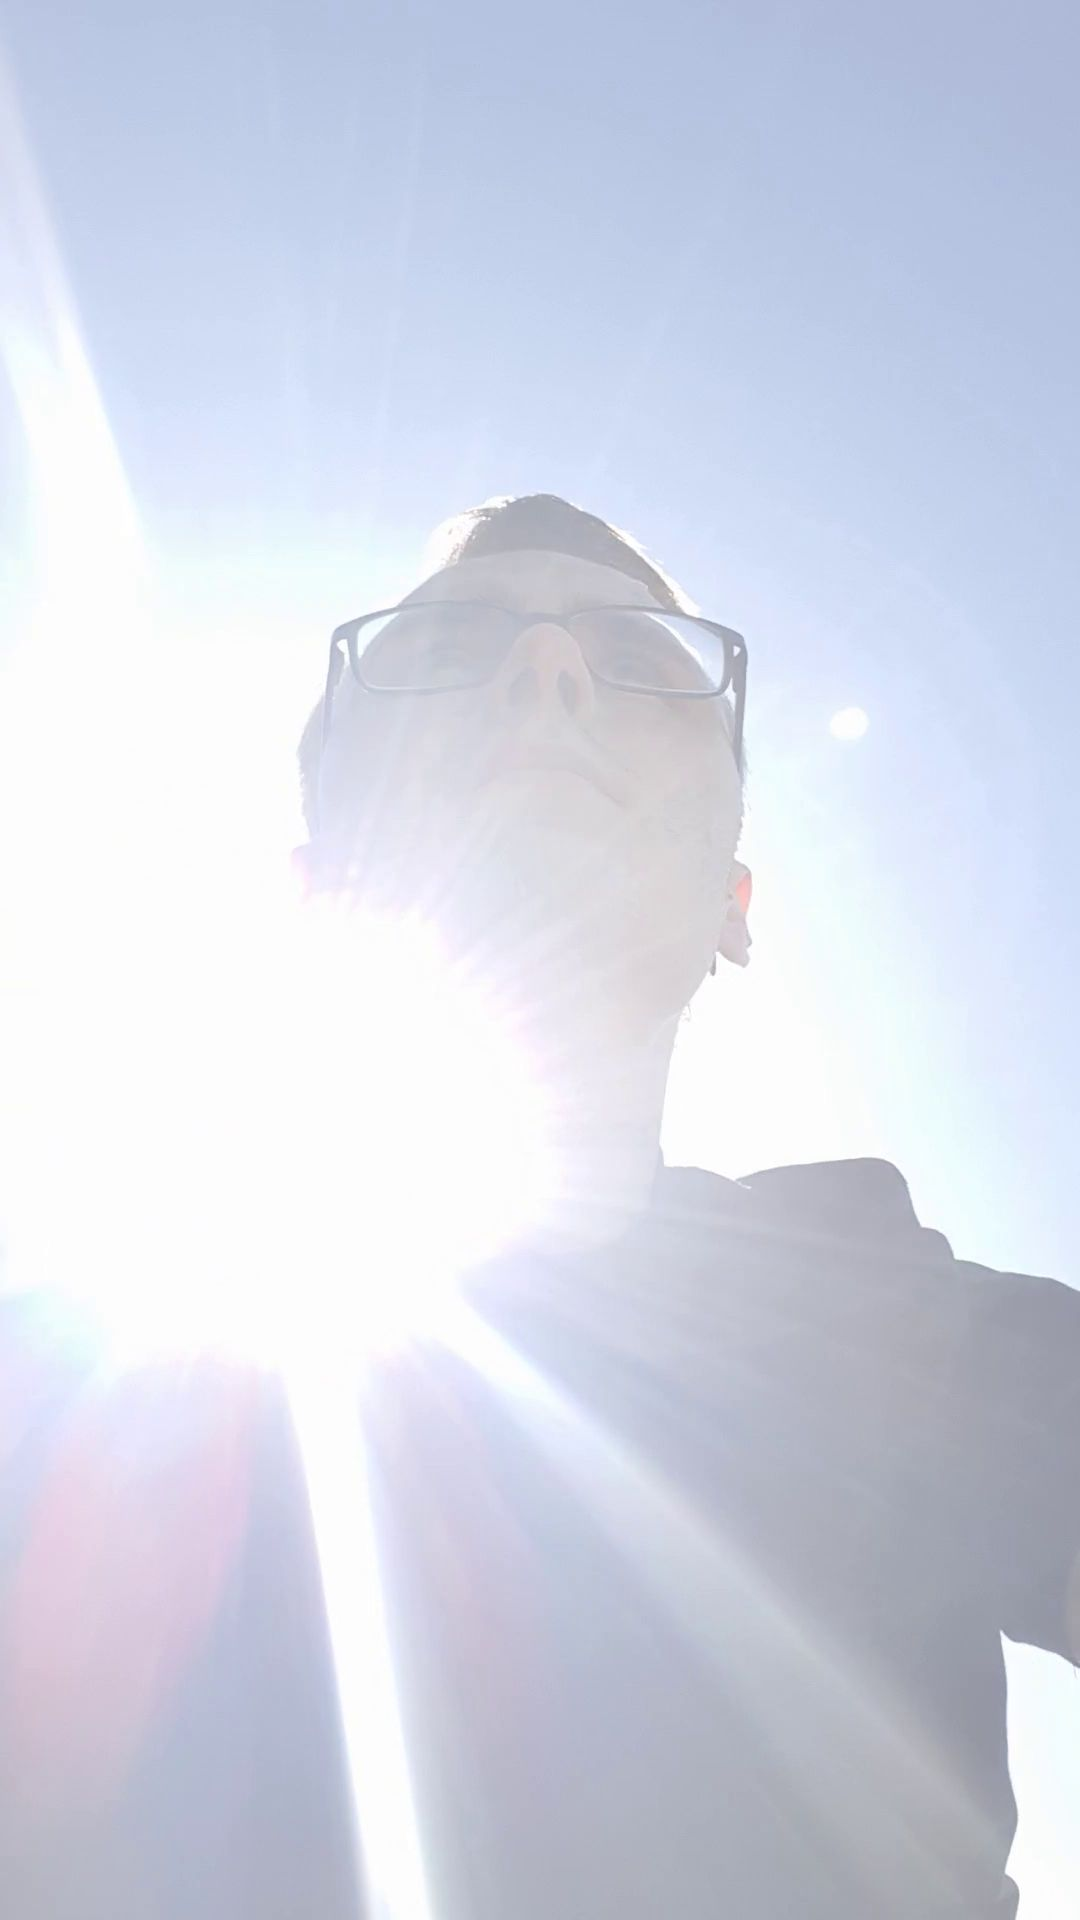
\includegraphics[width=\linewidth]{evaluation/face_error_bright.jpg}
        \caption{Beispiel für nicht erkanntes Gesicht wegen extremer Helligkeit.}
        \label{fig:evaluation:face:error:bright}
    \end{subfigure}
    \begin{subfigure}{0.3\textwidth}
        
\includegraphics[width=\linewidth]{evaluation/face_error_dark.jpg}
        \caption{Beispiel für nicht erkanntes Gesicht wegen extremer Dunkelheit.}
        \label{fig:evaluation:face:error:dark}
    \end{subfigure}
    \caption{Extreme Lichtverhältnisse, die das Erkennen von Gesichtern erschweren.}
    \label{fig:evaluation:face:score}
\end{figure}

Zusätzlich zu der bereits beschriebenen Auswertung wurde untersucht, welchen Einfluss der ermittelte Abstand des Gesichts zum Bildschirm $\distancefacecamera$ auf die Qualität der Gesichtserkennung hat. Dabei wurde festgestellt, dass ab einem bestimmten Grenzwert alle erkannten Gesichter als \textit{schlecht} eingestuft wurden, wie in Abbildung \ref{fig:evaluation:distance:total} zu sehen ist. Weiterhin wurde festgestellt, dass alle betroffenen Gesichter mit \dlib erkannt wurden, wie in Abbildung \ref{fig:evaluation:distance:model} zu sehen ist. Beispiele für solche erkannten Gesichter sind in Abbildung \ref{fig:evaluation:bad:distance} zu sehen. Diese Gesichter sollen daher bei der weiteren Betrachtung ignoriert werden. Der Grenzwert, den die Distanz $\distancefacecamera$ dabei nicht überschreiten darf, wurde anhand der Daten auf 1 festgelegt.

\begin{figure}
    \centering
    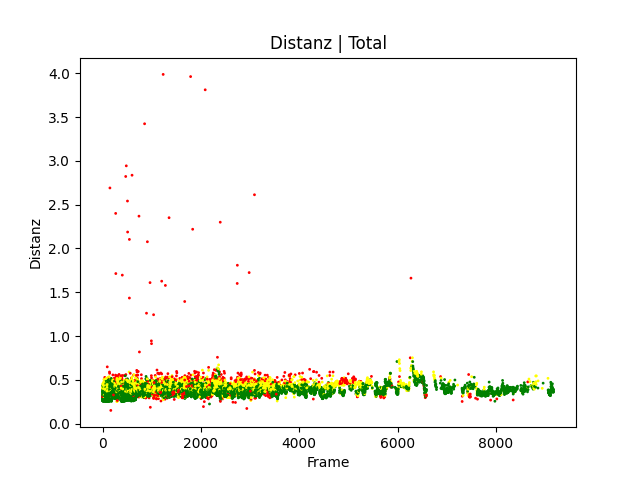
\includegraphics[width=0.7\linewidth]{evaluation/distance-total.png}
    \caption{Abhängigkeit der Qualität der Gesichtserkennung von der Distanz $\distancefacecamera$. Rot markiert sind die Gesichter, welche als \textit{schlecht erkannt} eingestuft wurden. Grün sind die Gesichter, die als \textit{gut erkannt} eingestuft wurden. Gelbe Punkte repräsentieren Gesichter, die als \textit{ungenau erkannt} eingestuft wurden.}
        \label{fig:evaluation:distance:total}
\end{figure}

\begin{figure}
    \centering
    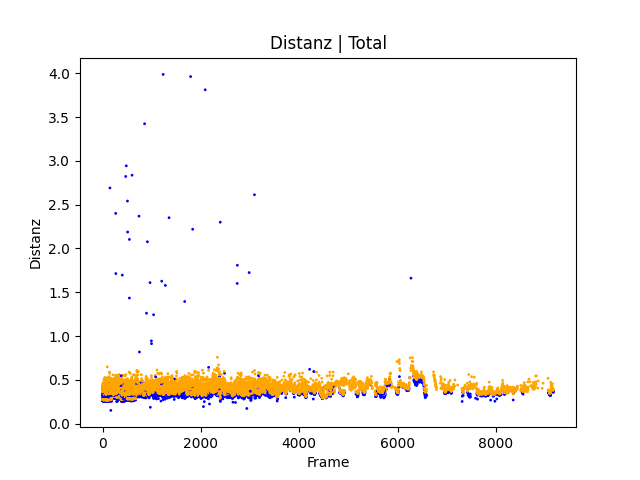
\includegraphics[width=0.7\linewidth]{evaluation/distance_model.png}
    \caption{Abhängigkeit der ermittelten Distanz $\distancefacecamera$ von der verwendeten Methode. Mit \dlib erkannte Gesichter werden blau dargestellt. Mit \mediapipe erkannte Gesichter werden orange dargestellt.}
    \label{fig:evaluation:distance:model}
\end{figure}



\begin{figure}[]
    \begin{subfigure}{0.425\textwidth}
        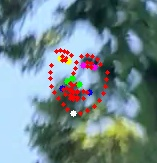
\includegraphics[width=\linewidth]{evaluation/bad_distance_1.jpg}
        \caption{Video 13, Frame 150, Distanz 2,69}
        \label{fig:evaluation:bad:distance:1}
    \end{subfigure}%
    \vspace{0.5cm}
    \begin{subfigure}{0.45\textwidth}
        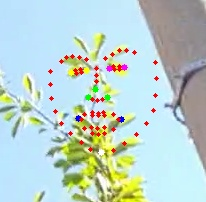
\includegraphics[width=\linewidth]{evaluation/bad_distance_2.jpg}
        \caption{Video 13, Frame 2739, Distanz 1,6}
        \label{fig:evaluation:bad:distance:2}
    \end{subfigure}
    \caption{Beispiele für Bilder, die als \textit{schlecht} eingestuft wurden und einen auffällig großen Abstand aufweisen.}
    \label{fig:evaluation:bad:distance}
\end{figure}

\subsection{Ergebnisse Blickrichtungsbestimmung}

Im Folgenden werden die Ergebnisse der Blickrichtungsbestimmung diskutiert. Dazu wird zunächst die Bestimmung der idealen Werte für die in Kapitel \ref{sec:implementation:gaze:interpretation} vorgestellte Seitenlänge $\hitthresholdsize$ und die Verschiebung $\hitthresholdposition$ beschrieben. Diese Werte werden für alle acht möglichen Kombinationen von Gesichtserkennung und Blickrichtungsbestimmung separat ermittelt. Basierend auf diesen Werten wird dann die Qualität der Blickrichtungsbestimmung für die einzelnen Videos analysiert, um zu untersuchen, wie gut verschiedene Umwelteinflüsse von den einzelnen Methoden zur Blickrichtungsbestimmung erkannt werden. Abschließend wird der Einfluss von geschlossenen Augen auf die Qualität der Blickrichtungsbestimmung diskutiert.

Generell wird für die Bewertung der Blickrichtung der F1-Score verwendet. Dazu wurde eine Ground Truth erstellt, die für jedes Bild angibt, ob die abgebildete Person auf das Smartphone schaut oder nicht. Als positive Instanzen werden alle Bilder verwendet, in denen die Person auf das Smartphone schaut (Kategorie A.1). Die negative Instanzen sind dann alle anderen Bilder, bei denen die Person nicht auf das Smartphone schaut (Kategorie A.0) oder bei denen das Gesicht der Person nicht im Bild erkenntlich ist (Kategorie A.2). Diese werden dann mit den Vorhersagen der einzelnen Methoden verglichen, um die \textit{True Positives} ($TP$), \textit{True Negatives} ($TN$), \textit{False Positives} ($FP$) und die \textit{False Negatives} ($FN$) zu ermitteln, anhand derer sich dann der F1-Score berechnet lässt. Aufgrund der Erkenntnisse aus Kapitel \ref{sec:evaluation:results:face} werden Bilder, bei denen das erkannte Gesicht einen Abstand von mehr als eins hat, bei der Berechnung des F1-Scores nicht berücksichtigt.

\subsubsection{Hyperparameter-Tuning}\label{sec:evaluation:results:gaze:threshold}

Um die idealen Werte für die Seitenlänge $\hitthresholdsize$ und die Verschiebung $\hitthresholdposition$ zu ermitteln, wurden zunächst erste Tests mit dem in Kapitel \ref{sec:evaluation:plan:tool} vorgestellten Anwendung zur Analyse der Daten durchgeführt, um ein grobes Intervall möglicher Werte für die Parameter $\hitthresholdsize$ und $\hitthresholdposition$ zu definieren. Dieser Test ergab die folgenden Intervalle:

\[
\hitthresholdsize \in [0,0.5] \qquad \hitthresholdposition \in [-0.1, 0.5]
\]

Diese Intervalle wurden in 50 gleich große Schritte unterteilt. Dann wurde für jede mögliche Kombination der Werte dieser Parameter der F1-Score für das Video berechnet. Diese wurden für jedes Video in einer Matrix gespeichert, wobei jede Kombination der Parameterwerte eine Zelle adressiert. Nach der Bearbeitung jedes Videos wurde der durchschnittliche F1-Score für alle diese Kombinationen berechnet. Ausgehend vom maximalen F1-Score wurden dann die Parameter $\hitthresholdsize$ und $\hitthresholdposition$ für jede mögliche Kombination von Gesichtserkennung und Blickrichtungsbestimmung ermittelt. 

Die aufgezeichneten Videos zeigen Faktoren, die bei der Analyse der Gesichtserkennung in Kapitel \ref{sec:evaluation:results:face} als hinderlich eingestuft wurden, die aber bei einer möglichen Studie im Rahmen der PrioBike-App beeinflusst werden können. So kann man den Teilnehmenden einer solchen Studie das Tragen von Sonnenbrillen verbieten. Des Weiteren hat man Einfluss auf die Tageszeit, zu der eine Studie stattfindet, weshalb extreme Dunkelheit in der Nacht vermieden werden kann. Daher wurde das oben beschriebene Verfahren erneut durchgeführt. Diesmal wurden jedoch einige Videos von der Betrachtung ausgeschlossen. Diese Videos waren:

\begin{itemize}
    \item Video 06, da \markus in diesem Video auf einer Bank sitzt und nicht auf dem Fahrrad,
    \item Video 07 und 10, da \paul und \philipp in diesen Videos eine Sonnenbrille tragen,
    \item Video 22, 23 und 24, da diese bei Nacht aufgenommen wurden.
\end{itemize}

Die besten Werte für die Parameter $\hitthresholdsize$ und $\hitthresholdposition$ der Blickrichtungsbestimmung mit Gesichtserkennung unter Verwendung von \dlib sind in den folgenden Abbildungen dargestellt:

\begin{itemize}
    \item  \textit{ETH-XGaze} in Abbildung  \ref{fig:evaluation:threshold:dlib:eth-gaze}
    \item  \textit{Gaze360} in Abbildung 
 \ref{fig:evaluation:threshold:dlib:l2cs-gaze-360}
    \item  \textit{MPIIFaceGaze} in Abbildung \ref{fig:evaluation:threshold:dlib:mpiifacegaze}
    \item  \textit{Kopfrotation} in Abbildung 
 \ref{fig:evaluation:threshold:dlib:head-rotation}
\end{itemize}

Für die Blickrichtungsbestimmung basierend auf der Gesichtserkennung mit \mediapipe sind die Parameter in den folgenden Abbildungen dargestellt:

\begin{itemize}
    \item  \textit{ETH-XGaze} in Abbildung \ref{fig:evaluation:threshold:mediapipe:eth-gaze}
    \item  \textit{Gaze360} in Abbildung \ref{fig:evaluation:threshold:mediapipe:l2cs-gaze-360}
    \item  \textit{MPIIFaceGaze} in Abbildung \ref{fig:evaluation:threshold:mediapipe:mpiifacegaze}
    \item  \textit{Kopfrotation} in Abbildung \ref{fig:evaluation:threshold:mediapipe:head-rotation}
\end{itemize}

Es ist zu beachten, dass zur Bestimmung dieser Werte größtenteils Videos verwendet wurden, die von derselben Person aufgenommen wurden. Auch wenn versucht wurde, in diesen Videos eine möglichst große Vielfalt darzustellen, können die ermittelten Parameter dadurch beeinflusst worden sein. Im Anhang sind die idealen Parameter und die entsprechenden maximalen F1-Scores aufgeführt, die speziell für jedes Video ermittelt wurden. 

In Tabelle \ref{tab:evaluation:results:gaze:best:f1} sind die maximalen F1-Scores für jede Kombination von Gesichtserkennung und Blickrichtungsbestimmung aufgeführt. Es ist zu erkennen, dass die Eliminierung von vermeidbaren Umwelteinflüssen den F1-Score für jede Kombination verbessert. Die einzige Ausnahme ist die Kombination aus \mediapipe mit \mpii. Generell ist zu erkennen, dass die Blickrichtungsbestimmung mit \mpii mit Abstand die schlechtesten Ergebnisse erzielte. Bei näherer Betrachtung der Daten fiel auf, dass mit \mpii der Schnittpunkt $\intersection$ bei jedem verarbeiteten Frame in der Nähe des Koordinatenursprungs liegt. Dies ist auch daran zu erkennen, dass die ermittelte Seitenlänge $\hitthresholdsize$ (siehe Abbildungen \ref{fig:evaluation:threshold:dlib:mpiifacegaze} und \ref{fig:evaluation:threshold:mediapipe:mpiifacegaze}) deutlich kleiner ist als bei den anderen Ansätzen. Daher wird in fast allen Bildern, in denen zuvor ein Gesicht erkannt wurde, festgestellt, dass die Person auf das Smartphone schaut. Dies ist auch in Abbildung \ref{fig:evaluation:gaze:mpiifacegaze} zu sehen. Diese zeigt die Ground Truth des Blickkontaktes, die Vorhersage des Blickkontaktes, die Qualität der erkannten Gesichter und ob ein Gesicht erkannt wurde.

\begin{figure}
    \centering
    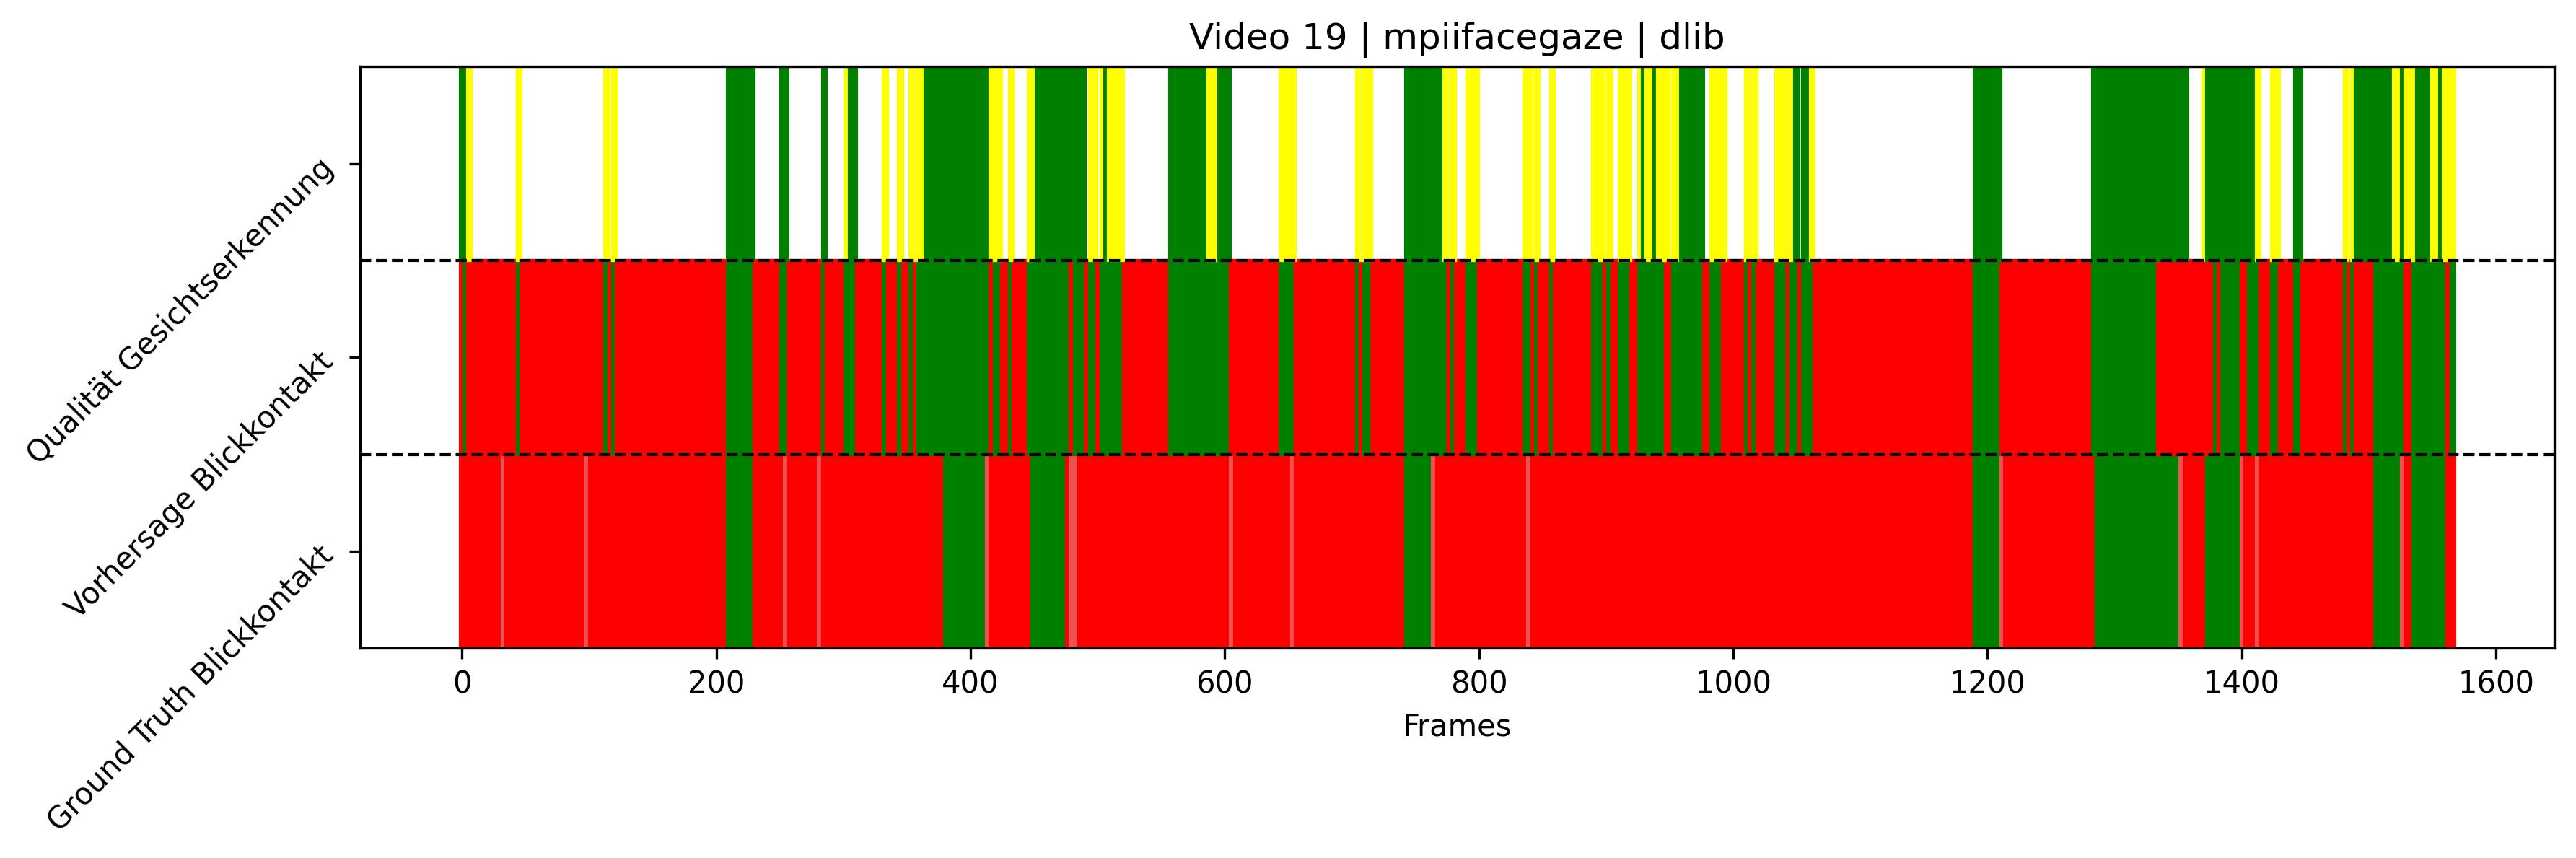
\includegraphics[width=\linewidth]{evaluation/19_dlib_mpiifacegaze.jpg}
    \caption{Übersicht über die Ground Truth des Blickkontakts, die Vorhersage des Blickkontakts und die Qualität der erkannten Gesichter. Bei der Gound Truth steht grün für die Kategorie A.1, rot für die Kategorie A.0 und rosa für die Kategorie A.2. Bei der Blickkontaktvorhersage bedeutet rot, dass die Person nicht auf das Smartphone schaut und grün, dass die Person auf das Smartphone schaut. Bei der Qualität der Gesichtserkennung steht rot für \textit{schlecht erkannt}, gelb für \textit{ungenau erkannt} und grün für \textit{gut erkannt}. Bilder, bei denen kein Gesicht erkannt wurde, werden nicht angezeigt. }
    \label{fig:evaluation:gaze:mpiifacegaze}
\end{figure}

Aufgrund der in Kapitel \ref{sec:evaluation:results:face} bestätigten Annahme, dass wenn kein Gesicht erkannt wird, die Person auch nicht auf das Smartphone schaut, erzielt dieser Ansatz bessere Ergebnisse, wenn nur in wenigen Bildern ein Gesicht erkannt wird. Da, wie in Kapitel \ref{sec:evaluation:results:face} gezeigt, \dlib generell weniger Gesichter erkennt, funktioniert der Ansatz mit \mpii am besten mit \dlib. Bereits bei der Konzeptentwicklung wurde vermutet, dass die Verwendung des \mpii-Datensatzes für die Bestimmung der Blickrichtung von Radfahrenden nicht geeignet ist, da der Datensatz nur Bilder von Personen enthält, die auf den Bildschirm eines Laptops schauen. Diese Vermutung konnte damit bestätigt werden.

Den mit Abstand besten F1-Score erreicht die Kombination aus Blickrichtungsbestimmung mit \ethg und Gesichtserkennung durch \mediapipe, direkt gefolgt von der Kombination aus \ethg und \dlib. Dies zeigt, dass der \ethg-Datensatz am besten geeignet ist, die Blickrichtung von Radfahrenden zu bestimmen. Der \gazed Datensatz erzielte ebenfalls gute Ergebnisse, wenn auch deutlich schlechter als der \ethg Datensatz. Weiterhin ist zu erkennen, dass die Blickrichtungsbestimmung aus der Kopfdrehung in Kombination mit \mediapipe ebenfalls gut für die Bestimmung der Blickrichtung von Radfahrenden geeignet ist.

\begin{table}[]
\begin{tabular}{l c c c c c}
\toprule
               & \textbf{Gesichtserkennung} & \textbf{ETH-XGaze} &\textbf{Gaze360}  & \textbf{MPIIFaceGaze} & \textbf{Kopfrotation} \\
\midrule
\multirowcell{2}{Alle Videos}   & dlib          & 0,855             & 0,732                & 0,686    & 0,703                     \\
                                & MediaPipe     & 0,874             & 0,708                & 0,493      & 0,797        \\
\midrule
\multirowcell{2}{Teilmenge\\der Videos} & dlib          & 0,91            & \textbf{0,848}        & \textbf{0,704}  & 0,729            \\
                                        & MediaPipe    & \textbf{0,928}    & 0,808                  & 0,439& \textbf{0,833}           \\
          \bottomrule
\caption{Maximaler durchschnittlicher F1-Score für die einzelnen Methoden zur Bestimmung der Blickrichtung mit unterschiedlicher Gesichtserkennungen als Grundlage.}
\label{tab:evaluation:results:gaze:best:f1}
\end{tabular}
\end{table}


\begin{figure}{}
    \begin{subfigure}{0.45\textwidth}
        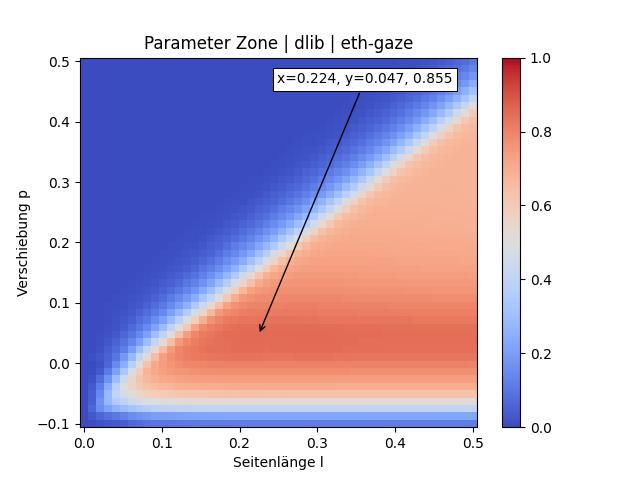
\includegraphics[width=\linewidth]{evaluation/dlib-eth-gaze-total-contour.jpg}
        \caption{Alle Videos}
        \label{fig:evaluation:threshold:dlib:eth-gaze:all}
    \end{subfigure}
    \begin{subfigure}{0.45\textwidth}
        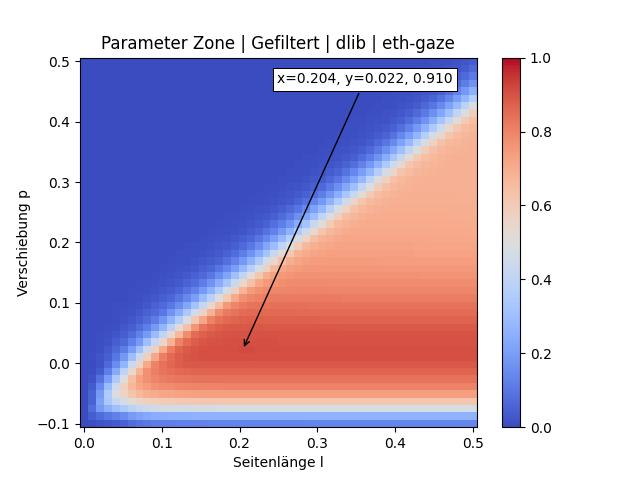
\includegraphics[width=\linewidth]{evaluation/dlib-eth-gaze-total-ignore-contour.jpg}
        \caption{Teilmenge der Videos}
        \label{fig:evaluation:threshold:dlib:eth-gaze:ignore}
    \end{subfigure}%
    \caption{Ergebnis des Hyperparameter-Tunings für die Gesichtserkennung mit \dlib und die Blickrichtungsbestimmung mit \ethg.}
    \label{fig:evaluation:threshold:dlib:eth-gaze}
\end{figure}
\begin{figure}{}
    \begin{subfigure}{0.45\textwidth}
        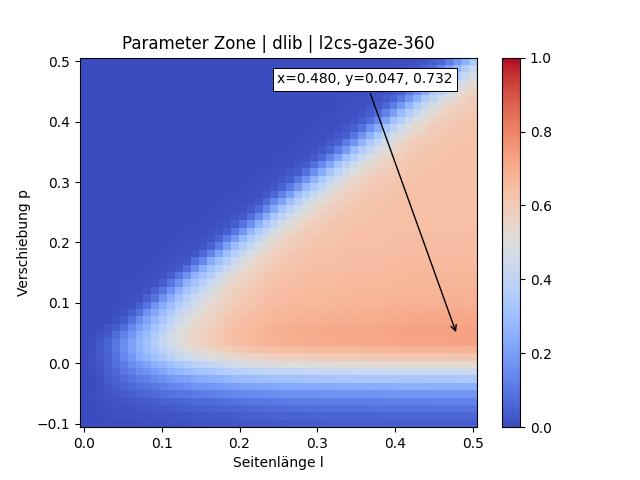
\includegraphics[width=\linewidth]{evaluation/dlib-l2cs-gaze-360-total-contour.jpg}
        \caption{Alle Videos}
        \label{fig:evaluation:threshold:dlib:l2cs-gaze-360:all}
    \end{subfigure}%
    \begin{subfigure}{0.45\textwidth}
        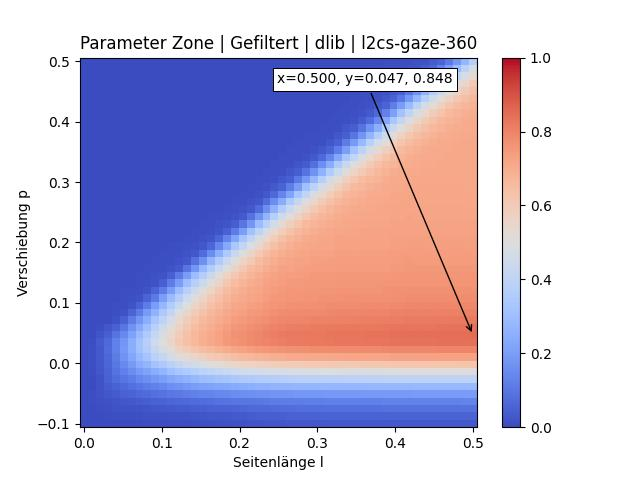
\includegraphics[width=\linewidth]{evaluation/dlib-l2cs-gaze-360-total-ignore-contour.jpg}
        \caption{Teilmenge der Videos}
        \label{fig:evaluation:threshold:dlib:l2cs-gaze-360:ignore}
    \end{subfigure}%
    \caption{Ergebnis des Hyperparameter-Tunings für die Gesichtserkennung mit \dlib und die Blickrichtungsbestimmung mit \gazed.}
    \label{fig:evaluation:threshold:dlib:l2cs-gaze-360}
\end{figure}
\begin{figure}{}
    \begin{subfigure}{0.45\textwidth}
        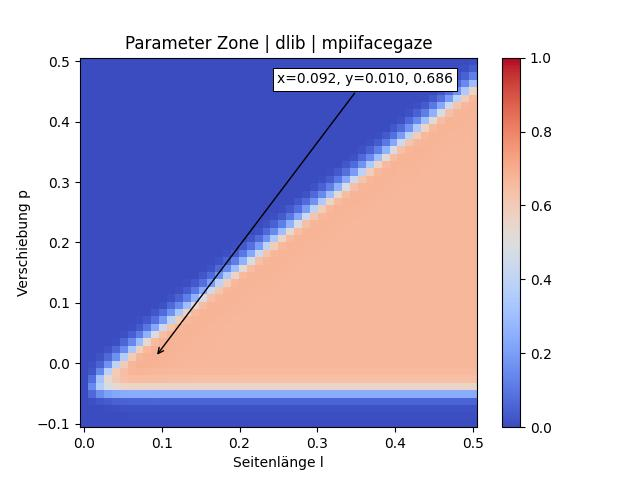
\includegraphics[width=\linewidth]{evaluation/dlib-mpiifacegaze-total-contour.jpg}
        \caption{Alle Videos}
        \label{fig:evaluation:threshold:dlib:mpiifacegaze:all}
    \end{subfigure}
    \begin{subfigure}{0.45\textwidth}
        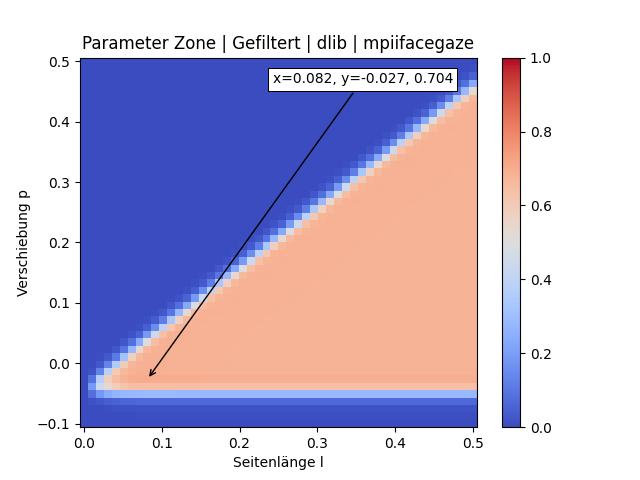
\includegraphics[width=\linewidth]{evaluation/dlib-mpiifacegaze-total-ignore-contour.jpg}
        \caption{Teilmenge der Videos}
        \label{fig:evaluation:threshold:dlib:mpiifacegaze:ignore}
    \end{subfigure}%
    \caption{Ergebnis des Hyperparameter-Tunings für die Gesichtserkennung mit \dlib und die Blickrichtungsbestimmung mit \mpii.}
    \label{fig:evaluation:threshold:dlib:mpiifacegaze}
\end{figure}
\begin{figure}{}
    \begin{subfigure}{0.45\textwidth}
        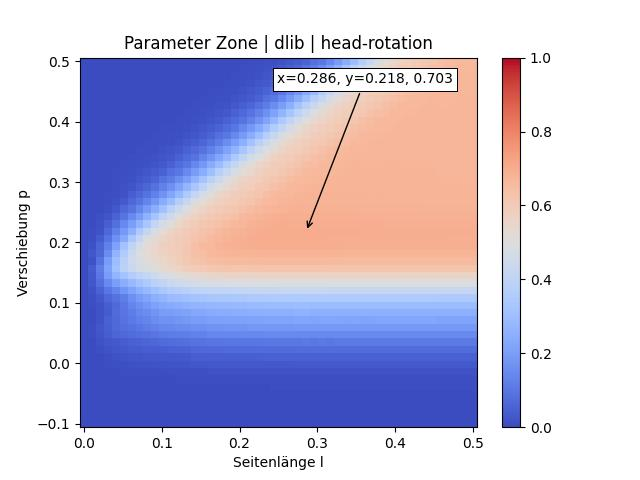
\includegraphics[width=\linewidth]{evaluation/dlib-head-rotation-total-contour.jpg}
        \caption{Alle Videos}
        \label{fig:evaluation:threshold:dlib:head-rotation:all}
    \end{subfigure}
    \begin{subfigure}{0.45\textwidth}
        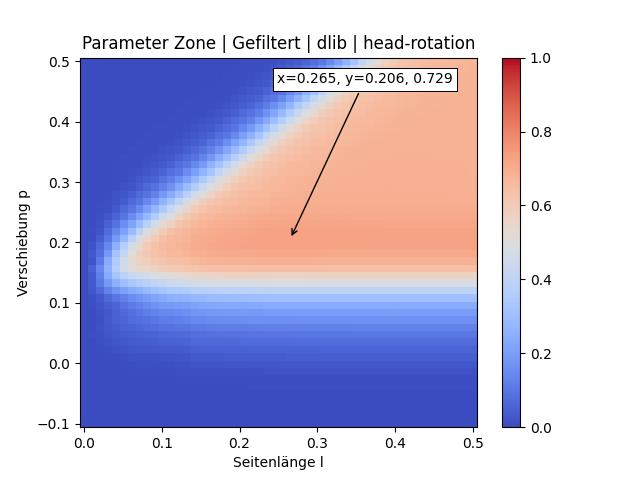
\includegraphics[width=\linewidth]{evaluation/dlib-head-rotation-total-ignore-contour.jpg}
        \caption{Teilmenge der Videos}
        \label{fig:evaluation:threshold:dlib:head-rotation:ignore}
    \end{subfigure}%
    \caption{Ergebnis des Hyperparameter-Tunings für die Gesichtserkennung mit \dlib und die Blickrichtungsbestimmung mittels der Kopfrotation.}
    \label{fig:evaluation:threshold:dlib:head-rotation}
\end{figure}

\begin{figure}{}
    \begin{subfigure}{0.45\textwidth}
        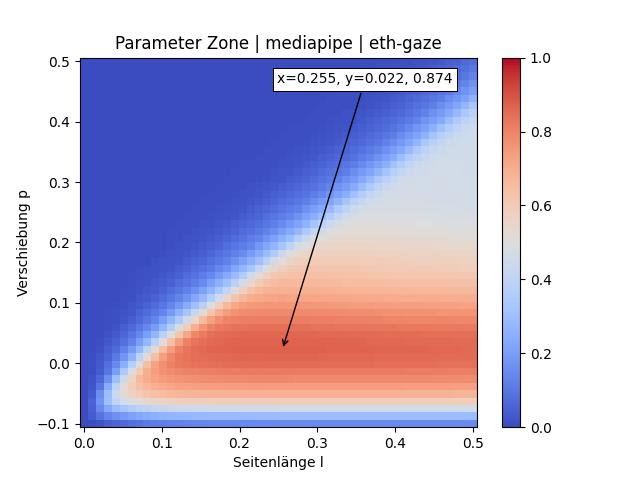
\includegraphics[width=\linewidth]{evaluation/mediapipe-eth-gaze-total-contour.jpg}
        \caption{Alle Videos}
        \label{fig:evaluation:threshold:mediapipe:eth-gaze:all}
    \end{subfigure}
    \begin{subfigure}{0.45\textwidth}
        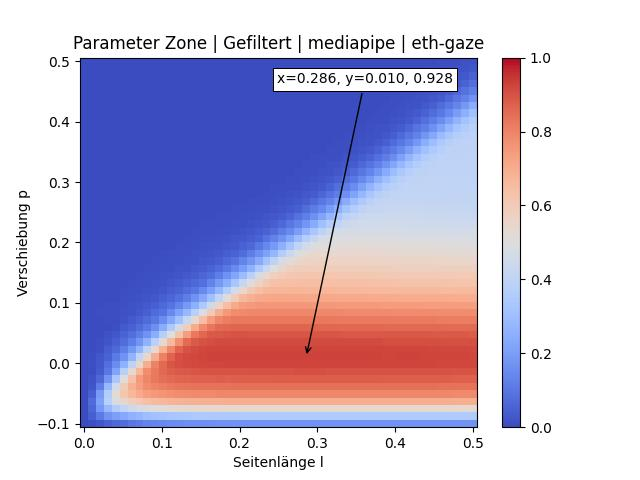
\includegraphics[width=\linewidth]{evaluation/mediapipe-eth-gaze-total-ignore-contour.jpg}
        \caption{Teilmenge der Videos}
        \label{fig:evaluation:threshold:mediapipe:eth-gaze:ignore}
    \end{subfigure}%
    \caption{Ergebnis des Hyperparameter-Tunings für die Gesichtserkennung mit \mediapipe und die Blickrichtungsbestimmung mit \ethg.}
    \label{fig:evaluation:threshold:mediapipe:eth-gaze}
\end{figure}
\begin{figure}{}
    \begin{subfigure}{0.45\textwidth}
        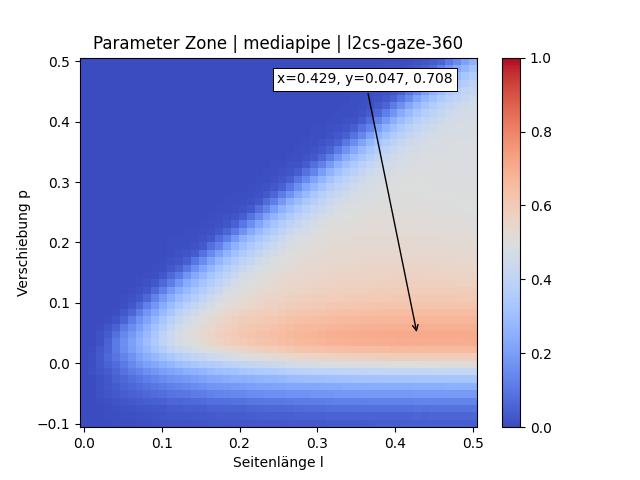
\includegraphics[width=\linewidth]{evaluation/mediapipe-l2cs-gaze-360-total-contour.jpg}
        \caption{Alle Videos}
        \label{fig:evaluation:threshold:mediapipe:l2cs-gaze-360:all}
    \end{subfigure}%
    \begin{subfigure}{0.45\textwidth}
        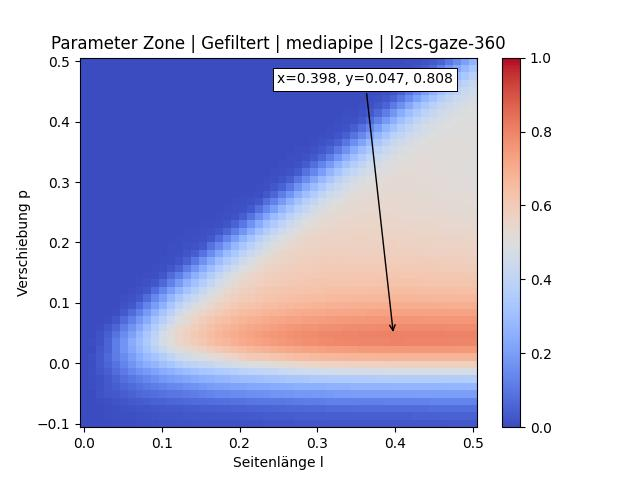
\includegraphics[width=\linewidth]{evaluation/mediapipe-l2cs-gaze-360-total-ignore-contour.jpg}
        \caption{Teilmenge der Videos}
        \label{fig:evaluation:threshold:mediapipe:l2cs-gaze-360:ignore}
    \end{subfigure}%
    \caption{Ergebnis des Hyperparameter-Tunings für die Gesichtserkennung mit \mediapipe und die Blickrichtungsbestimmung mit \gazed.}
    \label{fig:evaluation:threshold:mediapipe:l2cs-gaze-360}
\end{figure}
\begin{figure}{}
    \begin{subfigure}{0.45\textwidth}
        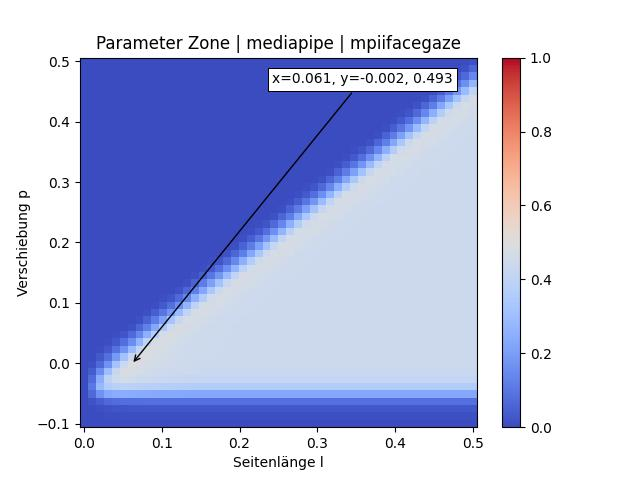
\includegraphics[width=\linewidth]{evaluation/mediapipe-mpiifacegaze-total-contour.jpg}
        \caption{Alle Videos}
        \label{fig:evaluation:threshold:mediapipe:mpiifacegaze:all}
    \end{subfigure}
    \begin{subfigure}{0.45\textwidth}
        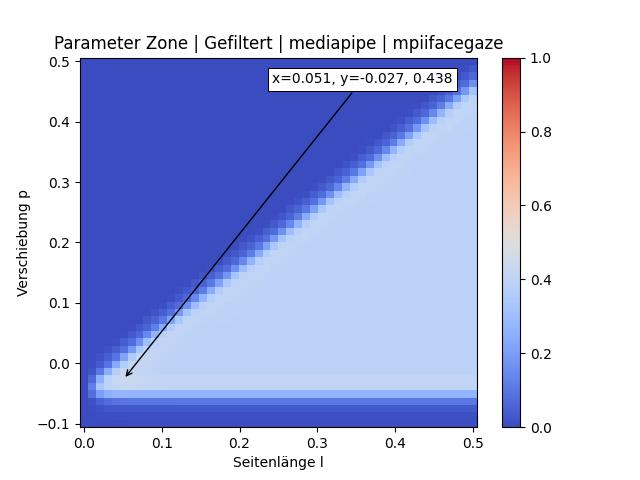
\includegraphics[width=\linewidth]{evaluation/mediapipe-mpiifacegaze-total-ignore-contour.jpg}
        \caption{Teilmenge der Videos}
        \label{fig:evaluation:threshold:mediapipe:mpiifacegaze:ignore}
    \end{subfigure}%
    \caption{Ergebnis des Hyperparameter-Tunings für die Gesichtserkennung mit \mediapipe und die Blickrichtungsbestimmung mit \mpii.}
    \label{fig:evaluation:threshold:mediapipe:mpiifacegaze}
\end{figure}
\begin{figure}{}
    \begin{subfigure}{0.45\textwidth}
        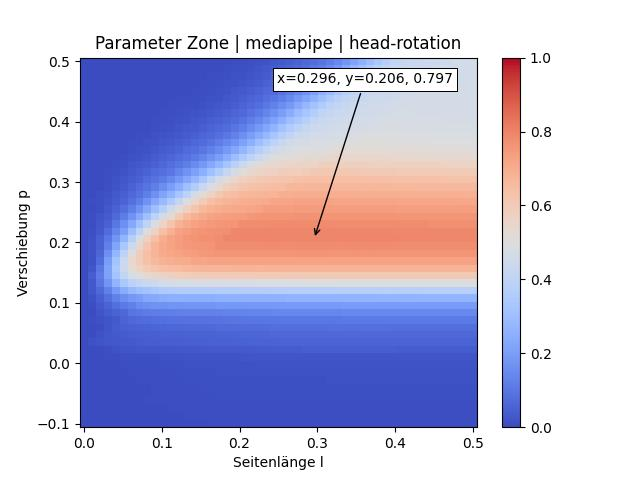
\includegraphics[width=\linewidth]{evaluation/mediapipe-head-rotation-total-contour.jpg}
        \caption{Alle Videos}
        \label{fig:evaluation:threshold:mediapipe:head-rotation:all}
    \end{subfigure}
    \begin{subfigure}{0.45\textwidth}
        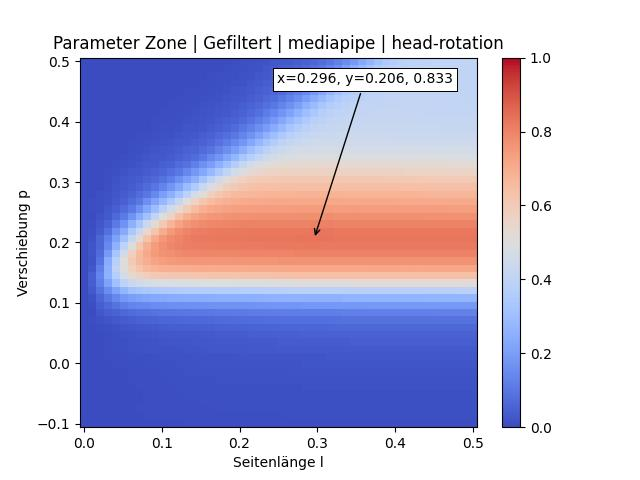
\includegraphics[width=\linewidth]{evaluation/mediapipe-head-rotation-total-ignore-contour.jpg}
        \caption{Teilmenge der Videos}
        \label{fig:evaluation:threshold:mediapipe:head-rotation:ignore}
    \end{subfigure}%
    \caption{Ergebnis des Hyperparameter-Tunings für die Gesichtserkennung mit \mediapipe und die Blickrichtungsbestimmung mittels der Kopfrotation.}
    \label{fig:evaluation:threshold:mediapipe:head-rotation}
\end{figure}

Betrachtet man die Diagramme in den Abbildungen \ref{fig:evaluation:threshold:dlib:eth-gaze} bis \ref{fig:evaluation:threshold:mediapipe:head-rotation} genauer, so scheint es, dass die Seitenlänge $\hitthresholdsize$ ab einem bestimmten Wert beliebig groß gewählt werden kann und dennoch ähnlich gute Ergebnissen erzielt werden. Bei der Vergrößerung von $\hitthresholdsize$ passiert vor allem, dass Schnittpunkte $\intersection$ von Personen, die links oder rechts neben das Smartphone schauen, als Blick auf das Smartphone interpretiert werden. Bereits in der Arbeit von Henseler \cite{bachelor:henseler:gaze-ebikes} konnte die Tendenz erkannt werden, dass, wenn Radfahrende ihren Blick vom Straßenverkehr abwenden, sie in fast allen Fällen auf das in der Halterung montierte Smartphone schauen. Von 1.516 Bildern schauten die Teilnehmenden der Studie von Henseler insgesamt nur vier Mal neben das Smartphone. Durch die scheinbar wirkungslose Vergrößerung der Seitenlänge $\hitthresholdsize$ ist diese Tendenz auch in den für diese Arbeit aufgenommenen Videos zu erkennen. Es ist daher zu beachten, dass je nach Wahl von $\hitthresholdsize$ Blicke links und rechts neben den Bildschirms nicht erkannt werden können. Dies wird unter anderem in Video 06 gezeigt. In diesem Video sitzt die dargestellte Person nicht auf dem Fahrrad, sondern ruht auf einer Bank. Dabei sieht die Person häufig links und rechts neben das Display des Smartphones. Die Ergebnisse des Hyperparameter-Tunings speziell für dieses Video sind in Abbildung \ref{fig:evaluation:threshold:daneben} dargestellt. Es ist zu erkennen, dass ab einer Seitenlänge von ca. 0,2 der F1-Score wieder abnimmt.

\begin{figure}
    \centering
    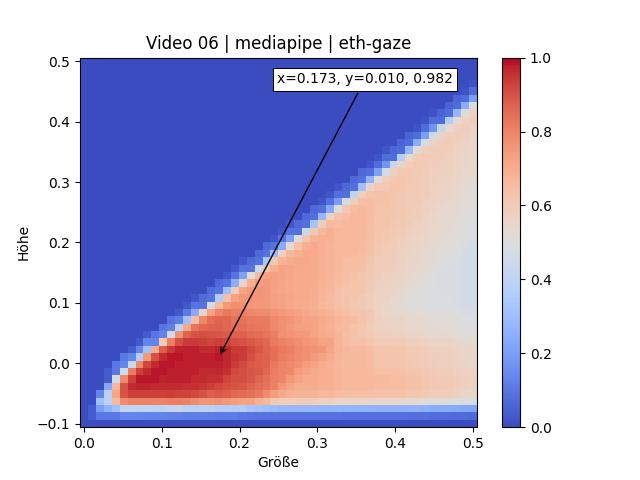
\includegraphics[width=0.6\linewidth]{evaluation/06-mediapipe-eth-gaze-contour.jpg}
    \caption{Ergebnisse des Hyperparameter-Tunings nur für Video 06.}
    \label{fig:evaluation:threshold:daneben}
\end{figure}

\subsubsection{Auswirkungen von Umwelteinflüssen auf die Blickrichtungsbestimmung}


Mittels der in Kapitel \ref{sec:evaluation:results:gaze:threshold} ermittelten Parameter $\hitthresholdsize$ und $\hitthresholdposition$ wurde für jedes Video der F1-Score berechnet, um die Leistungsfähigkeit der Ansätze unter verschiedenen Umgebungsbedingungen zu untersuchen. Es wurden die Parameter verwendet, die durch das Auslassen einiger Videos mit vermeidbaren Störfaktoren ermittelt wurden. Die Ergebnisse dieser Berechnung sind in Tabelle \ref{tab:evaluation:best:results} dargestellt. Im Anhang befindet sich eine detaillierte Auflistung der für den F1-Score erforderlichen Werte für alle Videos. 
\begin{table}[]
    \centering
    \begin{tabular}{c | c | c c c c}
    \toprule
        \textbf{Video} & \textbf{Gesichtsmodell} & \textbf{ETH-XGaze} & \textbf{Gaze360} & \textbf{MPIIFaceGaze} & \textbf{Kopfrotation} \\
        \hline
\multirow{2}{*}{01} & dlib & \cellcolor[HTML] {0DF200}\textcolor{black}{0,947} & \cellcolor[HTML] {10EE00}\textcolor{black}{0,93} & \cellcolor[HTML] {31CD00}\textcolor{black}{0,804} & \cellcolor[HTML] {3CC300}\textcolor{black}{0,765} \\ & MediaPipe & \cellcolor[HTML] {04FB00}\textcolor{black}{\textbf{0,983}} & \cellcolor[HTML] {34CB00}\textcolor{black}{0,794} & \cellcolor[HTML] {877800}\textcolor{white}{0,469} & \cellcolor[HTML] {28D700}\textcolor{black}{0,841} \\ \hline
\multirow{2}{*}{02} & dlib & \cellcolor[HTML] {0DF200}\textcolor{black}{\textbf{0,947}} & \cellcolor[HTML] {20DE00}\textcolor{black}{0,869} & \cellcolor[HTML] {45BA00}\textcolor{black}{0,73} & \cellcolor[HTML] {45BA00}\textcolor{black}{0,727} \\ & MediaPipe & \cellcolor[HTML] {0EF100}\textcolor{black}{0,943} & \cellcolor[HTML] {27D800}\textcolor{black}{0,846} & \cellcolor[HTML] {926D00}\textcolor{white}{0,429} & \cellcolor[HTML] {18E700}\textcolor{black}{0,903} \\ \hline
\multirow{2}{*}{03} & dlib & \cellcolor[HTML] {09F500}\textcolor{black}{0,959} & \cellcolor[HTML] {28D700}\textcolor{black}{0,843} & \cellcolor[HTML] {699500}\textcolor{black}{0,583} & \cellcolor[HTML] {48B700}\textcolor{black}{0,716} \\ & MediaPipe & \cellcolor[HTML] {06F900}\textcolor{black}{\textbf{0,973}} & \cellcolor[HTML] {718D00}\textcolor{white}{0,554} & \cellcolor[HTML] {C53A00}\textcolor{white}{0,227} & \cellcolor[HTML] {0EF100}\textcolor{black}{0,944} \\ \hline
\multirow{2}{*}{04} & dlib & \cellcolor[HTML] {0EF100}\textcolor{black}{\textbf{0,944}} & \cellcolor[HTML] {3BC300}\textcolor{black}{0,766} & \cellcolor[HTML] {7B8300}\textcolor{white}{0,518} & \cellcolor[HTML] {8F7000}\textcolor{white}{0,441} \\ & MediaPipe & \cellcolor[HTML] {0FF000}\textcolor{black}{0,938} & \cellcolor[HTML] {32CC00}\textcolor{black}{0,798} & \cellcolor[HTML] {986700}\textcolor{white}{0,405} & \cellcolor[HTML] {6C9300}\textcolor{black}{0,575} \\ \hline
\multirow{2}{*}{05} & dlib & \cellcolor[HTML] {10EF00}\textcolor{black}{0,936} & \cellcolor[HTML] {29D500}\textcolor{black}{0,834} & \cellcolor[HTML] {3FC000}\textcolor{black}{0,75} & \cellcolor[HTML] {38C700}\textcolor{black}{0,778} \\ & MediaPipe & \cellcolor[HTML] {01FD00}\textcolor{black}{\textbf{0,989}} & \cellcolor[HTML] {36C900}\textcolor{black}{0,786} & \cellcolor[HTML] {8D7100}\textcolor{white}{0,448} & \cellcolor[HTML] {27D800}\textcolor{black}{0,847} \\ \hline
\multirow{2}{*}{\textit{06}} & dlib & \cellcolor[HTML] {18E600}\textcolor{black}{\textbf{0,902}} & \cellcolor[HTML] {619E00}\textcolor{black}{0,62} & \cellcolor[HTML] {5FA000}\textcolor{black}{0,625} & \cellcolor[HTML] {807F00}\textcolor{white}{0,498} \\ & MediaPipe & \cellcolor[HTML] {38C600}\textcolor{black}{0,775} & \cellcolor[HTML] {4DB200}\textcolor{black}{0,697} & \cellcolor[HTML] {21DD00}\textcolor{black}{0,866} & \cellcolor[HTML] {7F8000}\textcolor{white}{0,5} \\ \hline
\multirow{2}{*}{\textit{07}} & dlib & \cellcolor[HTML] {A55900}\textcolor{white}{0,352} & \cellcolor[HTML] {A15E00}\textcolor{white}{0,368} & \cellcolor[HTML] {976800}\textcolor{white}{0,41} & \cellcolor[HTML] {A35C00}\textcolor{white}{0,363} \\ & MediaPipe & \cellcolor[HTML] {6C9300}\textcolor{black}{\textbf{0,574}} & \cellcolor[HTML] {AC5300}\textcolor{white}{0,325} & \cellcolor[HTML] {916E00}\textcolor{white}{0,431} & \cellcolor[HTML] {8C7300}\textcolor{white}{0,452} \\ \hline
\multirow{2}{*}{08} & dlib & \cellcolor[HTML] {4DB200}\textcolor{black}{\textbf{0,696}} & \cellcolor[HTML] {768900}\textcolor{white}{0,538} & \cellcolor[HTML] {E21D00}\textcolor{white}{0,115} & \cellcolor[HTML] {A95600}\textcolor{white}{0,337} \\ & MediaPipe & \cellcolor[HTML] {51AD00}\textcolor{black}{0,677} & \cellcolor[HTML] {51AE00}\textcolor{black}{0,681} & \cellcolor[HTML] {F50A00}\textcolor{white}{0,04} & \cellcolor[HTML] {728C00}\textcolor{white}{0,548} \\ \hline
\multirow{2}{*}{09} & dlib & \cellcolor[HTML] {17E800}\textcolor{black}{0,909} & \cellcolor[HTML] {0EF100}\textcolor{black}{0,942} & \cellcolor[HTML] {17E800}\textcolor{black}{0,908} & \cellcolor[HTML] {1FE000}\textcolor{black}{0,876} \\ & MediaPipe & \cellcolor[HTML] {2BD300}\textcolor{black}{0,829} & \cellcolor[HTML] {0BF300}\textcolor{black}{\textbf{0,955}} & \cellcolor[HTML] {46B900}\textcolor{black}{0,724} & \cellcolor[HTML] {1EE100}\textcolor{black}{0,881} \\ \hline
\multirow{2}{*}{\textit{10}} & dlib & \cellcolor[HTML] {59A500}\textcolor{black}{0,645} & \cellcolor[HTML] {837B00}\textcolor{white}{0,482} & \cellcolor[HTML] {936C00}\textcolor{white}{0,426} & \cellcolor[HTML] {1DE200}\textcolor{black}{0,886} \\ & MediaPipe & \cellcolor[HTML] {659A00}\textcolor{black}{0,604} & \cellcolor[HTML] {887700}\textcolor{white}{0,466} & \cellcolor[HTML] {817E00}\textcolor{white}{0,493} & \cellcolor[HTML] {10EF00}\textcolor{black}{\textbf{0,935}} \\ \hline
\multirow{2}{*}{11} & dlib & \cellcolor[HTML] {1EE100}\textcolor{black}{0,881} & \cellcolor[HTML] {28D700}\textcolor{black}{0,843} & \cellcolor[HTML] {48B700}\textcolor{black}{0,716} & \cellcolor[HTML] {46B900}\textcolor{black}{0,723} \\ & MediaPipe & \cellcolor[HTML] {0FF000}\textcolor{black}{\textbf{0,94}} & \cellcolor[HTML] {2ED100}\textcolor{black}{0,818} & \cellcolor[HTML] {9D6100}\textcolor{white}{0,386} & \cellcolor[HTML] {30CF00}\textcolor{black}{0,811} \\ \hline
\multirow{2}{*}{12} & dlib & \cellcolor[HTML] {0CF300}\textcolor{black}{0,951} & \cellcolor[HTML] {18E700}\textcolor{black}{0,906} & \cellcolor[HTML] {3DC200}\textcolor{black}{0,762} & \cellcolor[HTML] {3BC300}\textcolor{black}{0,768} \\ & MediaPipe & \cellcolor[HTML] {05FA00}\textcolor{black}{\textbf{0,978}} & \cellcolor[HTML] {37C800}\textcolor{black}{0,785} & \cellcolor[HTML] {AF5000}\textcolor{white}{0,313} & \cellcolor[HTML] {1CE300}\textcolor{black}{0,888} \\ \hline
\multirow{2}{*}{13} & dlib & \cellcolor[HTML] {12EC00}\textcolor{black}{0,922} & \cellcolor[HTML] {1DE200}\textcolor{black}{0,883} & \cellcolor[HTML] {2CD300}\textcolor{black}{0,826} & \cellcolor[HTML] {2BD300}\textcolor{black}{0,829} \\ & MediaPipe & \cellcolor[HTML] {0BF300}\textcolor{black}{\textbf{0,954}} & \cellcolor[HTML] {20DF00}\textcolor{black}{0,874} & \cellcolor[HTML] {897600}\textcolor{white}{0,461} & \cellcolor[HTML] {1DE200}\textcolor{black}{0,884} \\ \hline
\multirow{2}{*}{14} & dlib & \cellcolor[HTML] {3FC000}\textcolor{black}{0,754} & \cellcolor[HTML] {3FC000}\textcolor{black}{0,75} & \cellcolor[HTML] {4DB200}\textcolor{black}{0,698} & \cellcolor[HTML] {47B800}\textcolor{black}{0,719} \\ & MediaPipe & \cellcolor[HTML] {12EC00}\textcolor{black}{\textbf{0,925}} & \cellcolor[HTML] {47B800}\textcolor{black}{0,72} & \cellcolor[HTML] {9A6500}\textcolor{white}{0,396} & \cellcolor[HTML] {20DF00}\textcolor{black}{0,875} \\ \hline
\multirow{2}{*}{15} & dlib & \cellcolor[HTML] {02FC00}\textcolor{black}{\textbf{0,985}} & \cellcolor[HTML] {0EF100}\textcolor{black}{0,945} & \cellcolor[HTML] {1BE300}\textcolor{black}{0,891} & \cellcolor[HTML] {22DC00}\textcolor{black}{0,86} \\ & MediaPipe & \cellcolor[HTML] {02FC00}\textcolor{black}{\textbf{0,985}} & \cellcolor[HTML] {18E700}\textcolor{black}{0,905} & \cellcolor[HTML] {966900}\textcolor{white}{0,412} & \cellcolor[HTML] {0CF300}\textcolor{black}{0,953} \\ \hline
\multirow{2}{*}{16} & dlib & \cellcolor[HTML] {06F900}\textcolor{black}{\textbf{0,976}} & \cellcolor[HTML] {18E700}\textcolor{black}{0,905} & \cellcolor[HTML] {28D600}\textcolor{black}{0,837} & \cellcolor[HTML] {26D900}\textcolor{black}{0,851} \\ & MediaPipe & \cellcolor[HTML] {0CF300}\textcolor{black}{0,952} & \cellcolor[HTML] {11ED00}\textcolor{black}{0,927} & \cellcolor[HTML] {897600}\textcolor{white}{0,464} & \cellcolor[HTML] {0CF300}\textcolor{black}{0,952} \\ \hline
\multirow{2}{*}{17} & dlib & \cellcolor[HTML] {28D700}\textcolor{black}{0,843} & \cellcolor[HTML] {42BC00}\textcolor{black}{0,737} & \cellcolor[HTML] {29D500}\textcolor{black}{0,834} & \cellcolor[HTML] {30CE00}\textcolor{black}{0,807} \\ & MediaPipe & \cellcolor[HTML] {18E600}\textcolor{black}{\textbf{0,899}} & \cellcolor[HTML] {689700}\textcolor{black}{0,593} & \cellcolor[HTML] {32CC00}\textcolor{black}{0,799} & \cellcolor[HTML] {2FD000}\textcolor{black}{0,814} \\ \hline
\multirow{2}{*}{18} & dlib & \cellcolor[HTML] {18E700}\textcolor{black}{0,904} & \cellcolor[HTML] {20DE00}\textcolor{black}{0,868} & \cellcolor[HTML] {6D9200}\textcolor{black}{0,572} & \cellcolor[HTML] {56A900}\textcolor{black}{0,664} \\ & MediaPipe & \cellcolor[HTML] {14EB00}\textcolor{black}{\textbf{0,921}} & \cellcolor[HTML] {20DF00}\textcolor{black}{0,873} & \cellcolor[HTML] {B64900}\textcolor{white}{0,287} & \cellcolor[HTML] {20DE00}\textcolor{black}{0,871} \\ \hline
\multirow{2}{*}{19} & dlib & \cellcolor[HTML] {0BF300}\textcolor{black}{\textbf{0,956}} & \cellcolor[HTML] {10EF00}\textcolor{black}{0,935} & \cellcolor[HTML] {718D00}\textcolor{white}{0,552} & \cellcolor[HTML] {42BC00}\textcolor{black}{0,736} \\ & MediaPipe & \cellcolor[HTML] {0DF200}\textcolor{black}{0,946} & \cellcolor[HTML] {10EF00}\textcolor{black}{0,935} & \cellcolor[HTML] {936C00}\textcolor{white}{0,425} & \cellcolor[HTML] {27D800}\textcolor{black}{0,844} \\ \hline
\multirow{2}{*}{20} & dlib & \cellcolor[HTML] {10EE00}\textcolor{black}{0,932} & \cellcolor[HTML] {1DE200}\textcolor{black}{0,884} & \cellcolor[HTML] {35CA00}\textcolor{black}{0,79} & \cellcolor[HTML] {3CC300}\textcolor{black}{0,763} \\ & MediaPipe & \cellcolor[HTML] {10EE00}\textcolor{black}{\textbf{0,933}} & \cellcolor[HTML] {1EE100}\textcolor{black}{0,88} & \cellcolor[HTML] {699600}\textcolor{black}{0,588} & \cellcolor[HTML] {35CA00}\textcolor{black}{0,79} \\ \hline
\multirow{2}{*}{21} & dlib & \cellcolor[HTML] {0EF100}\textcolor{black}{0,945} & \cellcolor[HTML] {1CE300}\textcolor{black}{0,887} & \cellcolor[HTML] {32CC00}\textcolor{black}{0,799} & \cellcolor[HTML] {39C500}\textcolor{black}{0,772} \\ & MediaPipe & \cellcolor[HTML] {0EF100}\textcolor{black}{\textbf{0,945}} & \cellcolor[HTML] {2DD200}\textcolor{black}{0,821} & \cellcolor[HTML] {5DA200}\textcolor{black}{0,633} & \cellcolor[HTML] {38C600}\textcolor{black}{0,776} \\ \hline
\multirow{2}{*}{\textit{22}} & dlib & \cellcolor[HTML] {7D8200}\textcolor{white}{0,511} & \cellcolor[HTML] {FF0000}\textcolor{white}{0,0} & \cellcolor[HTML] {916E00}\textcolor{white}{0,43} & \cellcolor[HTML] {807F00}\textcolor{white}{0,498} \\ & MediaPipe & \cellcolor[HTML] {897600}\textcolor{white}{0,464} & \cellcolor[HTML] {FF0000}\textcolor{white}{0,0} & \cellcolor[HTML] {A35B00}\textcolor{white}{0,358} & \cellcolor[HTML] {689700}\textcolor{black}{\textbf{0,593}} \\ \hline
\multirow{2}{*}{\textit{23}} & dlib & \cellcolor[HTML] {42BC00}\textcolor{black}{0,737} & \cellcolor[HTML] {F30C00}\textcolor{white}{0,048} & \cellcolor[HTML] {8F7000}\textcolor{white}{0,439} & \cellcolor[HTML] {5DA200}\textcolor{black}{0,634} \\ & MediaPipe & \cellcolor[HTML] {2FD000}\textcolor{black}{0,816} & \cellcolor[HTML] {A55900}\textcolor{white}{0,353} & \cellcolor[HTML] {8F7000}\textcolor{white}{0,438} & \cellcolor[HTML] {2CD300}\textcolor{black}{\textbf{0,825}} \\ \hline
\multirow{2}{*}{\textit{24}} & dlib & \cellcolor[HTML] {25DA00}\textcolor{black}{\textbf{0,852}} & \cellcolor[HTML] {37C800}\textcolor{black}{0,782} & \cellcolor[HTML] {699500}\textcolor{black}{0,585} & \cellcolor[HTML] {2ED100}\textcolor{black}{0,817} \\ & MediaPipe & \cellcolor[HTML] {31CD00}\textcolor{black}{0,802} & \cellcolor[HTML] {6B9300}\textcolor{black}{0,58} & \cellcolor[HTML] {8E7100}\textcolor{white}{0,443} & \cellcolor[HTML] {2DD200}\textcolor{black}{0,822} \\ \hline

    \end{tabular}
    \caption{Übersicht über den F1-Score der einzelnen Videos in Abhängigkeit von $\hitthresholdsize$ und $\hitthresholdposition$. Aussortierte Videos sind kursiv dargestellt.}
    \label{tab:evaluation:best:results}
\end{table}

Mit \mpii wurden erwartungsgemäß keine guten Ergebnisse erzielt. Es ist jedoch zu erkennen, dass bis auf wenige Ausnahmen der F1-Score mit der Gesichtserkennung von \dlib deutlich besser ist als mit \mediapipe. Dies liegt, wie bereits erwähnt, daran, dass mit \mpii sehr viele \textit{False Positives} erkannt werden. Das liegt daran, dass Bilder ohne erkannte Gesichter als nicht auf das Smartphone schauend gewertet werden, und \dlib weniger Bilder erkennt als \mediapipe. So gibt es auch Videos, in denen die Blickrichtungsbestimmung mit \mpii sehr gut Ergebnisse erzielen konnte, wie zum Beispiel Video 09. Wie bereits im Kapitel \ref{sec:evaluation:results:face} erwähnt, ist \philipp in diesen Videos aus einem schwierigen Blickwinkel zu sehen, so dass nur Gesichter erkannt werden können, wenn die Person auf das Smartphone schaut.

Generell ist festzustellen, dass es Videos gibt, bei denen fast alle Methoden ein Problem haben. Dies sind vor allem die Videos mit vermeidbaren Störfaktoren (Videos 06, 07, 10, 22, 23 und 24). Diese schneiden schlechter ab, da sie bei der Berechnung der Parameter $\hitthresholdsize$ und $\hitthresholdposition$ nicht berücksichtigt wurden. Zusätzlich war der Grund, dass sie nicht beachtet wurden, dass mit diesen Störfaktoren generell weniger gute Ergebnisse erzielt werden konnten. Besonders schlecht schneiden Nacht-Videos 22, 23 und 24 ab. Dabei sind die Ergebnisse in Video 22 am schlechtesten. In den Videos 23 und 24, in denen die Beleuchtung stückweise besser wird, können auch bessere Ergebnisse erzielt werden. Besonders auffällig ist die schlechte Vorhersage von \gazed in Video 22. In diesem Video konnten keine \textit{True Positives} erkannt werden. Betrachtet man die Ergebnisse der Blickrichtungsbestimmung genauer, so fällt auf, dass der vorhergesagte Pitch- und Yaw-Winkel in diesen Fällen eine sehr große Abweichung von der tatsächlichen Blickrichtung aufweist, wie in Abbildung \ref{fig:evaluation:gaze:gaze360:error} zu sehen ist. Dies liegt daran, dass der \gazed Datensatz von Kellnhofer et al. \cite{paper:gaze360} keine Aufnahmen in dunkler Umgebung enthält. Auch wenn bei der Erstellung des Datensatzes Außenaufnahmen gemacht wurden, spiegeln diese nicht so dunkle Gesichter wider, wie sie in Video 22 zu sehen sind.



\begin{figure}
    \centering
    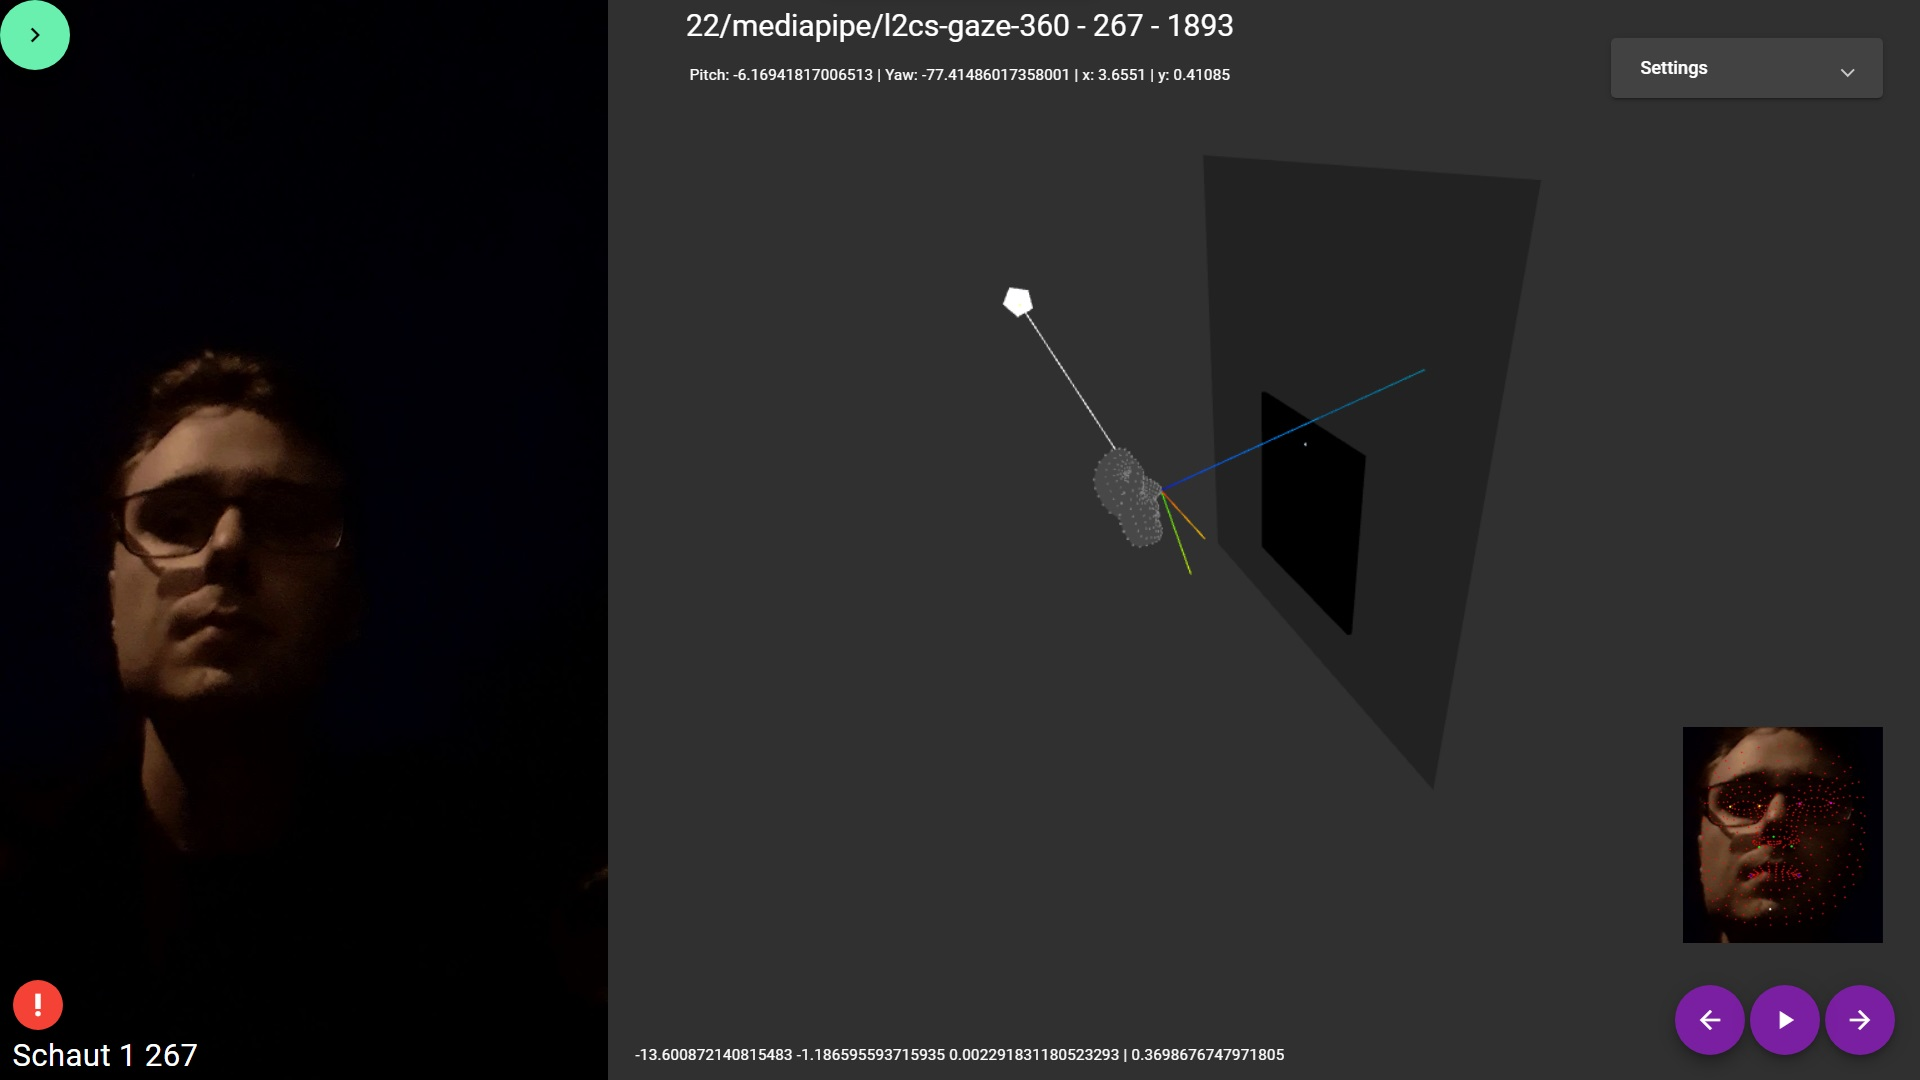
\includegraphics[width=0.9\linewidth]{evaluation/gaze360-error.jpg}
    \caption{Beispiel für die Blickrichtungsbestimmung mit \gazed bei Video 22. Es ist zu erkennen, dass der ermittelte Blickrichtungsvektor stark von der tatsächlichen Blickrichtung abweicht.}
    \label{fig:evaluation:gaze:gaze360:error}
\end{figure}

Weiterhin ist zu erkennen, dass die Verfahren zur Blickrichtungsbestimmung mit Convolutional Neural Networks in den Videos 07 und 10, in denen die dargestellten Personen eine Sonnenbrille tragen, Probleme haben.  Dagegen liefert die Blickrichtungsbestimmung mittels Kopfdrehung in Video 10 sehr gute Ergebnisse. Dies ist darauf zurückzuführen, dass die dargestellte Person in diesem Video, wie in Kapitel \ref{sec:evaluation:videos} beschrieben, den Kopf unnatürlich stark in Richtung des Smartphones neigt. In Video 07 hingegen kann auch mit der Kopfdrehung kein gutes Ergebnis erzielt werden. Dies ist jedoch auf das Auslassen der Videos bei der Bestimmung der Parameter zurückzuführen. Wie im Anhang in den Tabellen \ref{tab:appendix:07:local} (Video 07) und \ref{tab:appendix:10:local} (Video 10) zu sehen ist, werden bei der lokalen Berechnung der idealen Parameter mithilfe der Kopfdrehung jeweils die besten Ergebnisse mit einem F1-Score von 0,9 bzw. 0,977 erzielt.

Keine Auffälligkeiten zeigen hingegen die Videos, die durch Erschütterungen beeinträchtigt wurden (Video 04, 05, 12 und 13). Dies zeigt, dass Störfaktoren wie eine unebene Fahrbahnoberfläche von den Ansätzen gut kompensiert werden können. Auffällig ist auch, dass Video 14, das aufgrund der Sonne im Rücken der abgebildeten Person Probleme bei der Gesichtserkennung hatte, ebenfalls gute Ergebnisse erzielen konnte.

Es gibt jedoch ein Video, das keine besonderen Umgebungsbedingungen zeigt, für die Berechnung der Parameter verwendet wurde und dennoch schlechte Ergebnisse liefert. Es handelt sich um das Video 08 von \florian. Betrachtet man den bestmöglichen F1-Score, der bei der lokalen Berechnung der Parameter erzielt wurde (siehe Tabelle \ref{tab:appendix:08:local}), so fällt auf, dass dieser bei der Kombination von \mediapipe und \ethg mit 0,835 vergleichsweise niedrig ist. In allen anderen Videos, die keine Störfaktoren enthalten, liegt der F1-Score bei über 0,9. Daher wurde die Berechnung der lokalen Parameter des Videos genauer betrachtet. Dabei fiel auf, dass einige \textit{False Positives} in Momenten erkannt wurden, in denen \florian die Augen geschlossen hatte. Daher wurden die Bilder, in denen die Augen der Person geschlossen waren, aus der Betrachtung ausgeschlossen und die Parameterberechnung erneut durchgeführt. Wie in Abbildung \ref{fig:evaluation:threshold:mediapipe:eth-gaze:08} zu sehen ist, konnte der maximale F1-Score für das Video dadurch von 0,835 auf 0,944 verbessert werden. Dies zeigt, welchen Einfluss geschlossene Augen auf das Ergebnis haben können. Näheres dazu wird im folgenden Kapitel erläutert.

\begin{figure}{}
    \begin{subfigure}{0.45\textwidth}
        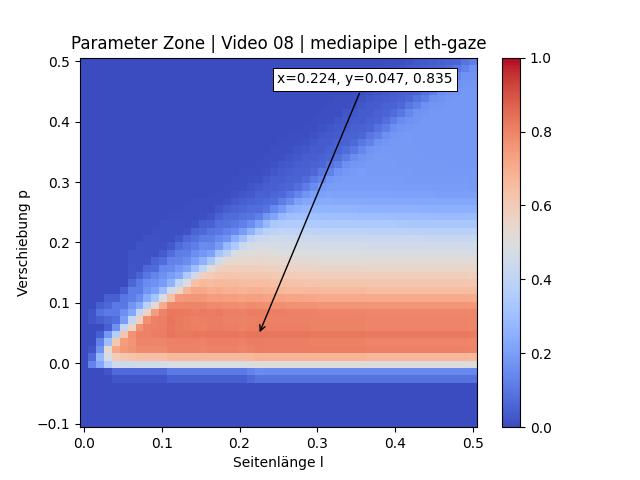
\includegraphics[width=\linewidth]{evaluation/08-mediapipe-eth-gaze-contour.jpg}
        \caption{Alle Bilder des Videos}
        \label{fig:evaluation:threshold:mediapipe:eth-gaze:08}
    \end{subfigure}
    \begin{subfigure}{0.45\textwidth}
        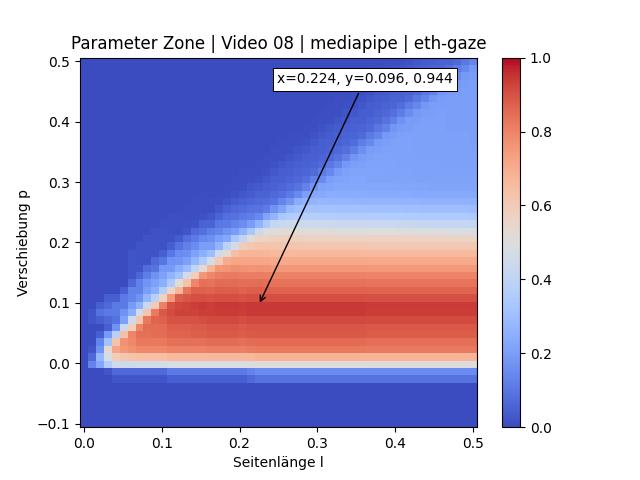
\includegraphics[width=\linewidth]{evaluation/08-mediapipe-eth-gaze-contour-without-blink.jpg}
        \caption{Nur Bilder mit geöffneten Augen}
        \label{fig:evaluation:threshold:mediapipe:eth-gaze:08:eye}
    \end{subfigure}%
    \caption{Ergebnis des Hyperparameter-Tunings basierend auf Video 08 mit Gesichtserkennung durch \mediapipe und Blickrichtungsbestimmung durch \ethg. Die Berechnung ist einmal mit allen Bildern des Videos in Abbildung \ref{fig:evaluation:threshold:mediapipe:eth-gaze:08} und einmal ohne Bilder, in denen die Augen der Person geschlossen waren, in Abbildung \ref{fig:evaluation:threshold:mediapipe:eth-gaze:08:eye} zu sehen.}
    \label{fig:evaluation:threshold:mediapipe:eth-gaze:08}
\end{figure}

\subsubsection{Auswirkung von geschlossenen Augen auf die Blickrichtungsbestimmung}\label{sec:evaluation:results:gaze:ear}

Teil des Konzepts der Blickrichtungsbestimmung mit Convolutional Neural Networks ist es, geschlossene Augen zu erkennen. Bilder mit geschlossenen Augen sollen, wie in Kapitel \ref{sec:concept:3d} beschrieben, bei der Bestimmung der Blickrichtung nicht beachtet werden. Im vorherigen Kapitel wurde bereits am Beispiel von Video 08 gezeigt, welchen Einfluss geschlossene Augen auf die Qualität der Blickrichtungsbestimmung haben können. Dies soll in diesem Kapitel weiter untersucht werden.

Als Grundlage wurde zunächst für jedes Bild untersucht, ob die Augen in diesem Bild geschlossen sind oder nicht, um eine Ground Truth zu erstellen. Im Kapitel \ref{tab:implementation:ear} wurde beschrieben, wie die Erkennung geschlossener Augen anhand der erkannten Gesichtsmerkmale um das Auge herum funktioniert. Dazu wird das \textit{Eye Aspect Ratio} \cite{paper:ear} für jedes erkannte Gesicht berechnet. Wie in Kapitel \ref{tab:implementation:ear} beschrieben, muss nun ein Grenzwert $\earthreshold$ bestimmt werden. Ist der $\ear$-Wert eines Gesichts kleiner als dieser Wert, werden die Augen als geschlossen betrachtet. 

Um den idealen Grenzwert zu bestimmen, wird der F1-Score verwendet. Die positiven Instanzen in diesem Fall sind alle Bilder mit geschlossenen Augen (Kategorie B.0). Die negativen Instanzen sind alle anderen Bilder. Anschließend wurde durch einen ersten Test ein Intervall ermittelt, in dem dieser Wert liegen muss:

\[
\earthreshold \in [0, 1]
\]

Dieses Intervall wird dann in 100 gleich große Schritte unterteilt. Jeder dieser Schritte wird als möglicher $\earthreshold$ angenommen, anhand dessen im Folgenden der F1-Score für jedes Video berechnet wird. Wie in Kapitel \ref{sec:evaluation:results:gaze:threshold}, wird auch diese Berechnung zweimal durchgeführt. Einmal mit allen Videos und einmal ohne die Videos mit vermeidbaren Störfaktoren wie Sonnenbrillen und dunkle Umgebungen bei Nacht. 

Die Ergebnisse sind in Tabelle \ref{tab:evaluation:ear} dargestellt. Es ist zu erkennen, dass mit diesem Ansatz geschlossene Augen nicht zuverlässig erkannt werden können. Der maximal erreichte F1-Score liegt bei 0,412. Gründe hierfür sind vor allem die schlechte Erkennung von Gesichtsmerkmalen um die Augen herum aufgrund der starken Kopfdrehung. Dadurch kann es vorkommen, dass die Gesichtspunkte ein geöffnetes Auge darstellen, obwohl das Auge in Wahrheit geschlossen ist. Außerdem wurde teilweise der Brillenrahmen als Auge erkannt, wie in Abbildung \ref{fig:evaluation:blink:false:positive} zu sehen ist, was zu einer falschen Erkennung eines geschlossenen Auges führt. Daher ist dieser Ansatz im Rahmen dieser Arbeit für die Erkennung geschlossener Augen nicht geeignet und wird daher für die weitere Auswertung nicht verwendet.

\begin{table}[]
    \centering
    \begin{tabular}{c | c c | c c}
        \toprule
        & \multicolumn{2}{c|}{\textbf{dlib}} &\multicolumn{2}{c}{\textbf{MediaPipe}} \\
        \midrule
        \textbf{Videos} & $\earthreshold$ & F1-Score & $\earthreshold$ & F1-Score \\
        \midrule
        Alle Videos & 0,183 & 0,325 & 0,165 & 0,362 \\
        Teilmenge der Videos & 0,173 & 0,362 & 0,159 & 0,412  \\
        \bottomrule
    \end{tabular}
    \caption{Maximaler mittlerer F1-Score für jede Methode mit Ausschluss der Bilder mit geschlossenen Augen im Vergleich zur Verarbeitung aller Bilder.}
    \label{tab:evaluation:ear}
\end{table}

\begin{figure}[]
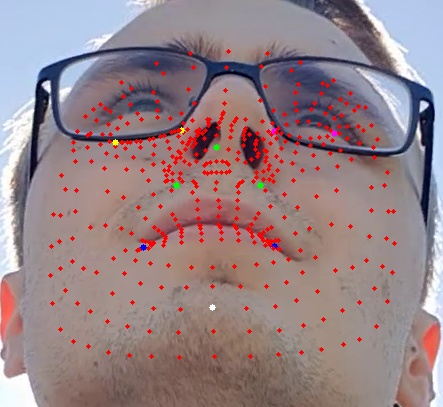
\includegraphics[width=0.5\linewidth]{evaluation/false_positive_blink.jpg}
\caption{Der Rahmen der Brille der Person wird als geschlossenes Auge erkannt.}\label{fig:evaluation:blink:false:positive}
\end{figure}

Da jedoch bereits in Video 08 gezeigt werden konnte, dass der F1-Score in diesem Video durch das Erkennen geschlossener Augen stark verbessert werden kann, soll untersucht werden, welche Verbesserung dadurch generell in den Videos erreicht werden kann. Dazu wurde das in Kapitel \ref{sec:evaluation:results:gaze:threshold} beschriebene Verfahren zur Bestimmung der idealen Parameter $\hitthresholdsize$ und $\hitthresholdposition$ erneut durchgeführt. Diesmal wurden jedoch die Bilder mit geschlossenen Augen anhand der Ground Truth erkannt und bei der Berechnung ignoriert. Die Ergebnisse sind in Tabelle \ref{tab:evaluation:blinks:filtered} dargestellt. Es ist zu erkennen, dass in allen Fällen der F1-Score durch das Erkennen der Augen verbessert werden konnte.

\begin{table}[]
\begin{tabular}{p{4cm} l c c c c}
\toprule
              &  & \textbf{ETH-XGaze} &\textbf{Gaze360}  & \textbf{MPIIFaceGaze} & \textbf{Kopfrotation} \\
\midrule
\multirowcell{2}{Teilmenge\\der Videos} & dlib          & 0,91            & 0,848    & 0,704  & 0,729            \\
                                        & MediaPipe    & 0,928    & 0,808                  & 0,439& 0,833          \\

\midrule
\multirowcell{2}{Teilmenge Videos ohne \\  geschlossene Augen} & dlib           & 0,920             & \textbf{0,855}          & \textbf{0,715} & 0,745                     \\
                                                            & MediaPipe      & \textbf{0,942}    & 0,817           & 0,450  & \textbf{0,846} \\               
\bottomrule
\caption{Darstellung der maximalen F1-Scores beim Aussortieren von Bildern mit geschlossen Augen. Zum Vergleich werden die F1-Scores aus Tabelle \ref{tab:evaluation:results:gaze:best:f1} gezeigt.}
\label{tab:evaluation:blinks:filtered}
\end{tabular}
\end{table}


\section{Zusammenfassung}

In diesem Kapitel wurde gezeigt, wie die Evaluation der erarbeiteten Konzepte durchgeführt wurde. Dazu wurden Videos von Radfahrenden in verschiedenen Situationen aufgenommen. Die Teilnehmenden wurden über das Ziel des Experiments informiert, was ihr Blickverhalten beeinflusst haben könnte. Die meisten Videos wurden von einer Person aufgenommen.

Zunächst wurde untersucht, wie gut die Gesichert der Radfahrenden mit \mediapipe und \dlib   erkannt werden können. Dabei zeigte sich, dass \mediapipe in deutlich mehr Bildern ein Gesicht erkennen konnte. Allerdings konnte auch mit \mediapipe in 9.546 von insgesamt 22.339 Bildern kein Gesicht erkannt werden. Es wurde jedoch gezeigt, dass in fast allen Fällen, in denen die Radfahrenden auf das Smartphone schauten, ein Gesicht erkannt werden konnte. Daraus kann geschlossen werden, dass wenn kein Gesicht erkannt wurde, die Person zu diesem Zeitpunkt nicht auf das Smartphone geschaut hat.

Als generelle Probleme bei der Gesichtserkennung konnten die Drehung des Kopfes, insbesondere entlang der Querachse, identifiziert werden. Weiterhin wurde festgestellt, dass extreme Lichtverhältnisse, z.B. bei Nacht, die Gesichtserkennung verschlechtern. 

Anschließend wurde die Blickrichtungsbestimmung ausgewertet. Dazu wurden für die Videos zunächst die Parameter $\hitthresholdsize$ und $\hitthresholdposition$ anhand der Ground Truth des Blickkontaktes bestimmt.  Dabei ist zu beachten, dass in den Videos zur Berechnung dieser Parameter hauptsächlich \markus zu sehen war. Die besten Ergebnisse wurden bei der Blickrichtungsbestimmung mit \ethg erzielt. Basierend auf der Gesichtserkennung von \mediapipe konnte ein F1-Score von 0,928 erreicht werden, bei \dlib waren es 0,91. Aber auch mit \gazed (0,848) und der Blickrichtungsbestimmung anhand der Kopfdrehung (0,833) konnten gute Ergebnisse erzielt werden. Weiterhin wurde gezeigt, dass der \mpii-Datensatz \cite{paper:mpiifacegaze} nicht für die Bestimmung der Blickrichtung von Radfahrern geeignet ist. Bei der Berechnung der Parameter wurde davon ausgegangen, dass keine im Rahmen der Studie beeinflussbaren Störfaktoren (Sonnenbrille, Tageszeit) in den Videos vorhanden sind.

Schließlich wurde der Einfluss geschlossener Augen auf die Ergebnisse untersucht. Es konnte festgestellt werden, dass die Erkennung geschlossener Augen die Ergebnisse aller Methoden zur Bestimmung der Blickrichtung verbessert. Der in dieser Arbeit implementierte Ansatz zur Erkennung geschlossener Augen lieferte jedoch nur sehr ungenaue Ergebnisse. Daher wurde dieser Ansatz für die weitere Auswertung nicht verwendet.












